\documentclass[a4paper,12pt]{article}
\usepackage{graphicx,epsfig}
\usepackage[english]{babel}
\usepackage{latexsym}
\usepackage{amssymb}
%\usepackage{sparticles} 	%Package for displaying sparticle names. 
%\usepackage{feynmf}		%Package for feynman diagrams. 
%% slashed symbols
\newcommand{\slashed}[1]{\hbox{{$#1$}\llap{$/$}}}

%%  !!!! Re-summed LV propagator and different cancellations
%%  !!!! ``shown in Fig. X, not shown in/on the Fig. X''

\begin{document}


%%
%% The title page
%% 
\begin{titlepage}
\renewcommand{\thefootnote}{\fnsymbol{footnote}}


\begin{flushright}
Requisites
\end{flushright}


\vfil

%%
%% Title itself
\begin{center}
\baselineskip20pt
{\bf \LARGE Dimension 5 Lorentz Violating operators in SQED}
\end{center}
\bigskip


\begin{center}
{\large\bf Abstract} \vspace*{.2cm}
\end{center}

\begin{quotation}
	Dimension five Lorentz Violating operators in SQED are reviewed.
	One loop RG running of these operators is analyzed. 
	The dimension 3 LV operators induced by soft SUSY breaking 
	are derived. 
	It is shown that Chern-Simons is never generated in this case. 
	Limits are set on the combinations of LV operators at the scale 
	below $ m_{soft} $.
	Dimension 6 LV operators in SQED/SQCD are listed.
\end{quotation}



\vfil
\end{titlepage}


\newpage

\setcounter{footnote}{0}
\setcounter{equation}{0}


%%%%%%%%%%%%%%%%%%%%%%%%%%%%%%%%%%%%%%%%%%%%%%
%%%%
%%%               Introduction
%%%%
%%%%%%%%%%%%%%%%%%%%%%%%%%%%%%%%%%%%%%%%%%%%%%
\section{Introduction}
\label{Intro}
	{\bf Note that this is not a proper section as yet.}

	One of the major questions concerned in this paper is the
	phenomenological implications of existence of the above
	operators. 
	When answering this question one must keep in mind that
	dimension 3 operators would dominate over the above ones.
	Even though dimension 3 operators are prohibited by
	supersymmetry [{\it a reference here}], they may be 
	{\it induced} by the above terms via:

	--- their equations of motion: 
	      ~~$ O^{(5)} \to m_e^2\, O^{(3)} $

	--- supersymmetry breaking:
		$ O^{(5)} \to m_{soft}^2\, O^{(3)} $

	--- both: \qquad\qquad~~~
		$ O^{(5)} \to (m_{soft}^2 + m_e^2)\, O^{(3)} $.

	The first ``mechanism'' is rather trivial and its effect
	is small compared to those of the others.
	The second and the third effects are dominating. 
	We will be dealing with them in section \ref{InducedDim3}.

	We also emphasize that the study of inducing dimension
	3 operators also raises the question of possibility of
	obtaining a Chern-Simons term. 
	Complete answer is found in section \ref{InducedDim3}
	discussing supersymmetry breaking.


%%%%%%%%%%%%%%%%%%%%%%%%%%%%%%%%%%%%%%%%%%%%%%
%%%%
%%%      Dimension 5 LV operators in SQED
%%%%
%%%%%%%%%%%%%%%%%%%%%%%%%%%%%%%%%%%%%%%%%%%%%%
\section{Dimension 5 LV operators in SQED}
\label{Dim5LV}
	Supersymmetric Quantum Electrodynamics (SQED) is described
	by two chiral superfields $ \Phi_+ $ and $ \Phi_- $, which
	are oppositely charged under the U(1) supersymmetry gauge
	group, and a gauge superfield $ V $: 
%%
%% The SQED lagrangian
\begin{eqnarray}
% first line
\nonumber
	\mathcal{L}_{\mathrm SQED} & =
&	
	\int d^4\theta\, 
	   \overline{\Phi}_+ e^{2eV} \Phi_+ ~~+~~
	\int d^4\theta\,
	   \Phi_- e^{-2eV} \overline{\Phi}_- ~~+~~ \\
% second line
\label{SQED}
& 
	+ &
	\frac{1}{16e^2} \int d^2\theta~
	WW ~~+~~
	\frac{1}{16e^2} \int d^2\overline{\theta}~
	\overline{WW} ~~+~~ \\
% third line
\nonumber
& 
	+ &
	\int \{\, d^2\theta~ m\, \Phi_-\Phi_+ ~+~
	         d^2\overline{\theta}~ 
		 m\, \overline{\Phi}_+\overline{\Phi}_-\,
             \}~~,
\end{eqnarray}
	where we denote 
  $ W_\alpha = - \frac{1}{16e^2} \overline{D}^2 
	e^{-2eV} D_\alpha\, e^{2eV} $ 
	as the fieldstrength
\footnote{
	Throughout this paper, we use notations of Wess and Bagger
\cite{Wess:1992cp}
	for chiral fermions and superfields.
	However, see Appendix 
\ref{app_conventions}	
	which summarizes these conventions, deviations from
	them and our adoptions.
	}.
	Here, 
%%
%% explaining notations
\begin{eqnarray*}
	d^4 \theta & = & d^2\theta\, d^2\overline{\theta} \\
	W W & = & W^\alpha W_\alpha \\
        \overline{W}\overline{W} & = & 
		\overline{W}_{\dot\alpha} \overline{W}^{\dot\alpha}
\end{eqnarray*}
	We shall call $ \Phi_+ $ ( $ \Phi_- $ ) the electron (positron) 
	superfield or just the electron and the positron (assuming charge
	$ + e = - | e | $ for the electron) for brevity.
	
	Supersymmetry and supersymmetric gauge invariance impose strong
	restrictions on the number of generic terms of specific mass
	dimension one can write.
	For the Lorentz-violating operators of dimension 5 in a 
	{\it massless} SQED, there can only be written three such terms.
	Because we generically take a {\it massive} SQED, we effectively
	add one more chiral field $ \Phi_- $, which thus allows us
	to write one more operator. 
	Adding a new chiral field does not add cross terms 
	$ \Phi_- \Phi_+ $ 
	within dimension 5 however
	(cross terms do arise within dimension 6, see 
	Section~\ref{Dim6}).
	In the matter sector, there is one operator for the electron and 
	a similar one for the positron
\footnote{
	Our notations in this paper for the background vectors differ
	from those of 
\cite{GrootNibbelink:2004za}.
	We use $ n $ with subscripts for the backgrounds, and 
	capital $ N_\pm $ for the emerging linear combinations of 
	them.}:
%%
%% the electron and positron operators
\begin{equation}
\label{LV_matter}
  \mathcal{L}_{\mathrm{LV}}^{\mathrm{matter}} = 
  \int d^4\theta \left\{ 
% electron
           \frac{i}{M} n_e^\mu\, \overline{\Phi}_+ e^{2eV} \nabla^+_\mu 
	                                                   \Phi_+ ~
% positron
	-~ \frac{i}{M} n_{\bar{e}}^\mu\, 
                          \Phi_- e^{-2eV} \nabla^-_\mu 
			  \overline{\Phi}_-
                 \right\}~.
\end{equation}
	The covariant derivatives are defined as
%% definition of nabla's
\[
          \nabla^\pm_\mu = - \frac{i}
                                  {4} \bar{\sigma}_\mu^{\dot{\alpha}\alpha}
	  	  \{ \nabla^\pm_\alpha 
		      \overline{\nabla}^\pm_{\dot{\alpha}} \} 
\]
\begin{eqnarray*}
        & \nabla^+_\alpha = e^{-2eV} D_\alpha e^{2eV}~~,
        & \overline{\nabla}^+_{\dot{\alpha}} = \overline{D}_{\dot{\alpha}} \\
        & \nabla^-_\alpha = D_\alpha~~,~~~~~~~~~~~~
        & \overline{\nabla}^-_{\dot{\alpha}} = e^{2eV} \overline{D}_{\dot{\alpha}}
                                    e^{-2eV}
\end{eqnarray*}
	The operators 
  (\ref{LV_matter})
	are parameterized by their external ``preferred''
	frames, $ n_e^\mu $ and $ n_{\bar{e}}^\mu $. 
	We chose the negative sign for the positron operator so that
	both operators transform into similar expressions:
%%                                 _
%% chiral operators in terms of D, D:
\begin{eqnarray*}
	\mathcal{L}_{\mathrm{LV}}^{\mathrm{matter}} & = 
  & {\displaystyle 
      \frac{n_e^\mu}
           {4 M}}
                   \overline{\sigma}_\mu^{\dot{\alpha}\alpha} \,
	           \overline{\Phi}_+ ~e^{2eV}\,\overline{D}_{\dot{\alpha}}\,
		    e^{-2eV} D_{\alpha} e^{2eV} \Phi_+ ~~+~~ \\
 & + & {\displaystyle
      \frac{n_{\bar{e}}^\mu}
           {4 M}}
                   \overline{\sigma}_\mu^{\dot{\alpha}\alpha} \,
                   \overline{\Phi}_- e^{-2eV} \overline{D}_{\dot{\alpha}}\,
                   e^{2eV} D_{\alpha} e^{-2eV} \Phi_- 
\end{eqnarray*}
	(here $ D_\alpha $ and $ \overline{D}_{\dot{\alpha}} $
	act all the way to the right).
	When doing loop calculations, these two expressions will produce
	identical vertices with a difference only in the sign of the
	charge.

	For the gauge supermultiplet (the photon, for brevity), 
	we get two operators.
	One of them is a Kahler term
%% photon -- Kahler term
\begin{equation}
\label{LV_gauge}
	\mathcal{L}_{\mathrm{LV}}^{\mathrm{gauge\ (K)}} =
        \int d^4\theta \, \overline{W \slashed{n}}W    ~~,
         ~~~~~ \bar{\slashed{n}}^{\dot{\alpha}\alpha} \equiv
               n^\mu \overline{\sigma}_\mu^{\dot{\alpha}\alpha}
\end{equation}
	parameterized by a background vector $ n^\mu $.
	It is the {\it only} term of dimension 5 within the gauge
	sector which is parameterized by a vector. 
	There is a different, superpotential term in the gauge
	sector
%% photon -- superpotential term
\begin{equation}
\label{LV_gauge_Tterm}
	\mathcal{L}_{\mathrm{LV}}^{\mathrm{gauge\ (T)}} =
	\int d^2\theta \, T^{\mu\nu\rho} \,
	        W \sigma_{\nu\rho} \partial_\mu W  + h.c.
\end{equation}
	which is parameterized by a third rank tensor 
  $ T^{\mu\nu\rho} $,
	antisymmetric in $(\nu\rho)$.
        This tensor can be expanded into irreducible components,
	in which case it would contain a purely irreducible
	3-tensor part antisymmetric in
	$(\nu\rho)$, and some vector parts.
	{\bf Check this statement better.}
	Uniqueness of the gauge operator (\ref{LV_gauge}) parameterized
	by an external vector within the set of operators of dimension
	5 then tells us (and this can be shown
	explicitly) that any such vector (i.e. ``reducible'') part of 
	the operator (\ref{LV_gauge_Tterm}) will reduce down to
	the form of the operator operator (\ref{LV_gauge}).
	Thus reducible parts of $ T^{\mu\nu\rho} $ can be
	absorbed into the operator (\ref{LV_gauge}).
	In order to obtain an operator stand-alone from the Kahler
	operator (\ref{LV_gauge}) we must take
  $ T^{\mu\nu\rho} $
	irreducible, i.e.
%% irreducibility of the tensor T
\begin{eqnarray*}
	T_\mu^{\phantom{\mu}\mu\rho} & = & 0 \\
	\epsilon_{\mu\nu\rho\sigma}\, T^{\nu\rho\sigma} & = & 0~.
\end{eqnarray*}

	Note that an operator 
(\ref{LV_gauge_Tterm}) 
	cannot exist in a non-abelian theory. 
	In the latter case, $ W_\alpha $'s are not gauge invariant,
	but are gauge covariant.
	Thus, to maintain gauge invariance of the operator, the
	partial derivative $ \partial_\mu $ in 
	(\ref{LV_gauge_Tterm}) would have to be replaced by
	a covariant derivative $ \nabla_\mu^+ $. 
	Then, the chirality property of the integrand is lost,
	and we can not write it as a superpotential term any longer.

	The set of operators (\ref{LV_matter}), (\ref{LV_gauge}) and
	(\ref{LV_gauge_Tterm}) is a complete set of Lorentz violating
	operators of dimension 5 in SQED.
	Here we present them in the component form in the Wess-Zumino
	gauge.
	The matter operator (\ref{LV_matter}) for the electron
	takes the form
%%
%% The electron LV operator in components with Weyl spinors; 
%% totally unresolved
\begin{eqnarray}
% the 1st line
\nonumber
\lefteqn{
   \frac{n_e^\mu}
        {M} \int d^4\theta\, \overline{\Phi}_+ e^{2eV} 
		\nabla_\mu^+ \Phi_+ = 
   \frac{\overline{\slashed{n}}_e^{\dot{\alpha}\alpha}}
	{4 M} \int d^4\theta\, \overline{\Phi}_+ e^{2eV} 
	\{ \overline{\nabla}_{\dot{\alpha}}^+ \nabla_\alpha^+ \} \Phi_+ = 
	}\\
% the 2nd line
\nonumber
&&
 = \frac{n^\mu}{M} \Bigg [~
    i \bar{F}_+ \mathcal{D}_\mu F_+ ~~+~~
    i e \bar{z}_+ D \mathcal{D}_\mu z_+ ~~-~~
    i e \mathcal{D}_\mu(\bar{z}_+) D z_+ ~~+~~ \\
% the 3rd line
\label{LV_electron_comp}
&&
  + ~~ 
    i e \frac{\sqrt{2}}{2} \left\{
               \overline{\psi_+\sigma^\mu}\lambda F_+ 
	       ~-~
               \overline{F_+\lambda\sigma^\mu} \psi_+
                         \right\} ~~+~~ 
    \frac{1}{2} e \overline{\psi_+\sigma^\mu}D\psi_+ ~~+~~\\
% the 4th line
\nonumber
&&
    +~~
    e^2 \bar{z}_+ \left\{
               \lambda\sigma^\mu\bar{\lambda} 
	       ~-~
               \overline{\lambda\sigma^\mu}\lambda 
                       \right\} z_+ 
  ~~-~~ \\
% the 5th line
\nonumber
&&
    -~~ 
    \frac{\sqrt{2}}{2} e \left\{ 
                      \overline{\psi_+\sigma^\nu}\sigma^\mu 
                     \bar{\lambda}\mathcal{D}_\nu z_+ +
                     \mathcal{D}_\nu(\bar{z}_+)\lambda\sigma^\mu
                     \bar{\sigma}^\nu \psi_+
                     \right \}
 ~~-~~ \\
% the 6th line
\nonumber
&&
 -~~
   \sqrt{2} e \left\{ 
                     \mathcal{D}_\mu(\overline{\psi_+)\lambda} z_+ 
		     ~+~ 
                     \bar{z}_+ \lambda \mathcal{D}_\mu \psi_+ 
                     \right\} 
 ~~+~~ 
  \frac{1}{2}\bar{\psi}_+\mathcal{D}_{(\mu}\mathcal{D}_{\nu)}
               \bar{\sigma}^\nu \psi_+ 
   ~~-~~ \\
% the 7th line
\nonumber
&&
   -~~
  \frac{1}{4} e \bar{\psi}_+\epsilon^{\mu\nu\rho\sigma}
              F_{\rho\sigma} \bar{\sigma}_\nu \psi_+
   ~~+~~
  i \bar{z_+} \mathcal{D}^\nu \mathcal{D}_\mu \mathcal{D}_\nu z_+ 
   ~~+~~
   \frac{1}{2} i e \mathcal{D}_\nu (\bar{z}_+) \epsilon^{\mu\nu\rho\sigma}
              F_{\rho\sigma} z_+ \, 
   \Bigg] ~,
\end{eqnarray}
        where the gauge derivative $ \mathcal{D}_\mu $ is 
$$ 
  \mathcal{D}_\mu = \partial_\mu + i\, e v_\mu~~.
$$
	The positron part of (\ref{LV_matter}) is obtained from
	(\ref{LV_electron_comp}) by changing ``+'' subscripts to
	``--'', and changing sign of all components of the vector
	superfield $ V $, see Appendix \ref{app_reduction} for
	more details.

	The gauge Kahler LV operator (\ref{LV_gauge}) reads in
	components as
%%
%% gauge Kahler term in components
\begin{eqnarray}
\label{LV_gauge_comp}
\lefteqn{
	\mathcal{L}_{\mathrm{LV}}^{\mathrm{gauge\ (K)}} =  
	\int d^4\theta \, \overline{W \slashed{n}}W ~=~
	} \\
% second line of this operator
\nonumber
	& = &
	2\, \overline{\lambda\,\slashed{n}}\, \Box\, 
	   \lambda 
	~+~
	2\, \lambda\, n^\mu \partial_\mu \slashed{\partial}\, 
	   \overline{\lambda} 
	~-~ 
	2\, D\, n_\mu \partial_\nu F^{\mu\nu}
	~+~ 
	\partial_\lambda F^{\lambda\mu}\, 
	\widetilde{F}_{\mu\nu} \cdot n^\nu
	~.
\end{eqnarray}

	Finally, the tensor operator (\ref{LV_gauge_Tterm}) is
%%
%% gauge Tensor term in components
\begin{eqnarray}
\nonumber
\lefteqn{
	\mathcal{L}_{\mathrm{LV}}^{\mathrm{gauge\ (T)}}  ~=~ 
	\int d^2\theta \, T^{\mu\nu\rho} \,
	        W \sigma_{\nu\rho} \partial_\mu W  ~+~ h.c. ~=~ } \\
% second line of this operator
	&&
\label{LV_gauge_Tterm_comp}	
	\quad
	=~
	\left\{ T^{\mu\nu\rho} 
		~+~ 
	       i\,\frac{1}{2}\,\epsilon^{\nu\rho\sigma\tau}
	       T^\mu_{\phantom{\mu}\sigma\tau} \right\} \times 
	\\
% third line of this operator
\nonumber
	&&
	\times
	\Biggl(
	     2i\, \overline{\lambda}\, \partial_\mu\partial_\nu
	     \overline{\sigma}_\rho\, \lambda 
		~+~
		\partial_\mu D\, \widetilde{F}_{\nu\rho}
		~-~
		\frac{1}{2}
		\left\{
			F_{\sigma\nu} ~+~ 
			i \widetilde{F}_{\sigma\nu}
		\right\}\, 
		\partial_\mu F_\rho^{\phantom{\rho}\sigma}
	\Biggr) 
	~+~ h.c.
\end{eqnarray}
	We notice here that this operator actually depends on
	a ``self-dual'' combination
\[
	T^{\mu\nu\rho} 
	~+~ 
	\frac{1}{2}\,i\,\epsilon^{\nu\rho\sigma\tau}
	T^\mu_{\phantom{\mu}\sigma\tau} 
\]
	rather than just on $ T^{\mu\nu\rho} $ itself. 
	This combination is invariant under
\[
	T^{\mu\nu\rho} 
	~\to~
	\frac{1}{2}\,i\,\epsilon^{\nu\rho\sigma\tau}
	T^\mu_{\phantom{\mu}\sigma\tau} 
	~.
\]
	This is rather natural, since the LHS of 
	(\ref{LV_gauge_Tterm_comp}) obeys the same property:
\[
	\frac{1}{2}\,i\,\epsilon^{\mu\nu\rho\sigma}
		\sigma_{\rho\sigma} = \sigma^{\nu\rho}~.
\]
	
	As mentioned in the Introduction, the above dimension 5 
	operators also induce dimension 3 LV operators via
	equations of motion or via supersymmetry breaking. 

	Dimension 3 operators can be limited experimentally
	much stronger then dimension 5 ones.
	Using renormalization group, however, allows us to
	extend the limits put on the dimension 3 operators
	to the dimension 5 ones via RG flow mixing. 
	According to our scenario, LV operators are generated
	at the UV scale $ M $, whereas experimental constraints
	can only be put at low energies.
	In order to apply them, we need to evolve the LV operators
	down to the low energy scale.
	To take into account the supersymmetry breaking, we will
	evaluate the LV operators at the soft supersymmetry
	breaking scale.

%%%%%%%%%%%%%%%%%%%%%%%%%%%%%%%%%%%%%%%%%%%%%%
%%%%
%%%      RG evolution of the LV operators
%%%%
%%%%%%%%%%%%%%%%%%%%%%%%%%%%%%%%%%%%%%%%%%%%%%
\section{RG evolution of the LV operators}
\label{RGEvolution}
	In this section we study how the LV operators introduced
	in section \ref{Dim5LV} evolve down the scale under
	the RG equations.
	It will certainly be useful to find out which operators mix
	with each other and which operators run independently.

	Loop calculations of this section, as well as of the
	following sections can be very efficiently simplified 
	by facilitating the ``vertex calculation property''.
	Using a simple observation, one can show that some
	parts of different diagrams cancel each other. 
	However, this property is remarkable also due to another
	reason: it shows that {\it tadpoles do not arise due
	to Lorentz-violation by operators of dimension 5}. 
	If existent, a tadpole 
\begin{equation}
\label{tadpole}
	\emph{A FIGURE OF A TADPOLE HERE}
\end{equation}
	would generate the $ D $ field {\bf with a quadratic divergency?}.
	This would lead to a catastrophe, since a non-zero VEV for $ D $ 
	will generate a disastrous mass to the scalar field:
%%
%% the mass term for the scalar field due to D,
%% see W&B, Eq.(7.10)
\begin{equation}
\nonumber
	\mathcal{L}_{SQED} ~\supset~ 
	\frac{e}
	     {2}\,
	D
	\left\{
		\overline{z}_+ z_+
		~-~
		\overline{z}_- z_-
	\right\}~.
\end{equation}
	The vertex cancellation property however, tells us that
	the tadpole diagram (\ref{tadpole}) is not modified due to
	Lorentz violation to any order, and thus vanishes provided the
	sum of charges of the theory is zero, 
	see Appendix~\ref{app_cancellation} for the details.

	It is important to mention here that it is enough to
	consider a massless SQED.
	The case of massive SQED will be partly studied in 
	section~\ref{Massive_SUSY}.
	But it is rather clear 
	that including mass at the first order of $ m^2 $
	can only {\it decrease} the power of the operators being
	generated at the loop level, and thus will not affect
	the renormalization of the dimension 5 operators themselves.
	{\bf Need to affirm this statement.}

Fig.~\ref{diag_LV_chiral}
	shows the diagrams contributing to the renormalization
	of the electron/positron operators at one loop level.
%%
%% one loop chiral (by LV insertion) diagrams; unbroken SUSY; massless 
%%
\begin{figure}[h]
\caption{\label{diag_LV_chiral}
        1-loop corrections to the
	chiral operators (\ref{LV_matter}). 
	Solid line denotes the chiral propagator, wiggled line
	represents the gauge superfield propagator, crossed circle
	represents an insertion of the LV operators
	(\ref{LV_matter}), (\ref{LV_gauge}).
}
\begin{center}
\begin{tabular}{ccc}
\includegraphics[width=2.7cm,height=2.7cm,keepaspectratio]{diag_chiral_A.ps}
&
\includegraphics[width=2.7cm,height=2.7cm,keepaspectratio]{diag_chiral_B.ps}
&
\includegraphics[width=2.7cm,height=2.7cm,keepaspectratio]{diag_chiral_C.ps} 
\end{tabular}

\begin{tabular}{rl}
\includegraphics[width=2.7cm,height=2.7cm,keepaspectratio]{diag_chiral_D.ps}
&
\includegraphics[width=2.7cm,height=2.7cm,keepaspectratio]{diag_chiral_E.ps}
\end{tabular}
\end{center}
\end{figure}

	The ({\it the cross LV sign here}) is the LV vertex arising 
	from (\ref{LV_matter}) or (\ref{LV_gauge}) where appropriate.
	Contributions of the operator (\ref{LV_gauge_Tterm}) we will
	consider later. 

	All diagrams in this section should actually have a subscript
	$ ``+'' $ or $ ``-'' $ 
	relating them to the corresponding supermultiplets.
	However, as is easy to see, all these diagrams are proportional
	to the {\it square} of the charge of the multiplet.
	So it is enough to consider only one set of diagrams keeping in 
	mind that the second set is obtained from the first one by a 
	trivial replacement of tags: $ ``+'' \to ``-'' $. 

	The operator (\ref{LV_gauge}) gets one loop corrections from 
	the diagrams shown in 
Fig.~\ref{diag_LV_gauge}.
%%
%% gauge (by LV insertion) diagrams; unbroken SUSY; massless 
%%
\begin{figure}[h]
\caption{\label{diag_LV_gauge}
        1-loop corrections to the gauge LV operator 
	$ \overline{W\slashed{n}} W $.
}
\begin{center}
\begin{tabular}{cccc}
\includegraphics[width=2.7cm,height=2.7cm,keepaspectratio]{diag_gauge_A.ps}
&
\includegraphics[width=2.7cm,height=2.7cm,keepaspectratio]{diag_gauge_B.ps}
&
\includegraphics[width=2.7cm,height=2.7cm,keepaspectratio]{diag_gauge_C.ps} 
&
\includegraphics[width=2.7cm,height=2.7cm,keepaspectratio]{diag_gauge_D.ps}
\end{tabular}
\begin{tabular}{cc}
\includegraphics[width=2.7cm,height=2.7cm,keepaspectratio]{diag_gauge_E.ps}
&
\includegraphics[width=2.7cm,height=2.7cm,keepaspectratio]{diag_gauge_F.ps}
\end{tabular}
\end{center}
\end{figure}
	(Note that in SQED gauge operators (\ref{LV_gauge}) or
	(\ref{LV_gauge_Tterm}) do not renormalize due to themselves
	due to the same reason why in ordinary QED the photon does not
	run due to itself).
	
	Here it is worth making some remarks.
	First, we note that it appears that it is only the operator
	(\ref{LV_gauge}) that gets contributions shown in
Fig.~\ref{diag_LV_gauge},
	and not the tensor operator (\ref{LV_gauge_Tterm}).
	An evident explanation for that is that one cannot form
	an irreducible 3-rank tensor out of a single vector
	$ n_e^\mu $ (or $ n_{\bar{e}}^\mu $).

	Another observation is that all quadratic divergencies in the
	diagrams of 
Figs.~\ref{diag_LV_chiral},~\ref{diag_LV_gauge}
	cancel. 
	In particular, this shows that a Chern-Simons term does not
	get generated by Lorentz violation at one loop at
	{\it exact SUSY} in massless SQED.

	Now we turn to the operator (\ref{LV_gauge_Tterm}).
	It is natural to expect that this operator should be 
	``stand-alone'', due to irreducibility of the tensor
	$ T^{\mu\nu\rho} $. 
	As mentioned above, diagrams in
Fig.~\ref{diag_LV_gauge}
	show that it does not get any contributions. 
	The diagram in
Fig.~\ref{diag_LV_gauge_Tterm}
%%
%% gauge (by LV insertion) diagrams; unbroken SUSY; massless 
%%
\begin{figure}[h]
\caption{\label{diag_LV_gauge_Tterm}
        1-loop corrections to the matter operators (\ref{LV_matter})
	due to the tensor operator (\ref{LV_gauge_Tterm}).
	The box symbolizes the insertion of the operator
	(\ref{LV_gauge_Tterm}).
}
\begin{center}
\includegraphics[width=2.7cm,height=2.7cm,keepaspectratio]{diag_chiral_T.ps}
\end{center}
\end{figure}
	gives a contribution of this operator to the matter
	LV ones. 
	In that figure, ({\emph sign of box}) is the insertion of the 
	operator
	(\ref{LV_gauge_Tterm}).
	The contribution of this diagram vanishes if 
	$ T^{\mu\nu\rho} $
	is irreducible.
	Thus, indeed, this operator does not mix with others and
	runs only due to the wavefunction renormalization. 
	
	The renormalization group equation following from the loop diagrams 
	in
Figs.~\ref{diag_LV_chiral},~\ref{diag_LV_gauge}
	reads as:
%%
%% Undiagonalized RG equation
%%
\begin{equation}
\label{RG_eqn_undiag}
     \mu \frac{\partial}
              {\partial\mu} 
                \left(
		\begin{array}{c}
                   n^\mu \\ 
		   n_e^\mu \\
                   n_{\bar{e}}^\mu \\
		   T^{\mu\nu\rho}
                \end{array} \right) = 
     \frac{e^2}
          {8 \pi^2} 
     \left(\begin{array}{rrrr}
                    2 & -1 & -1 & 0 \\
		   -6 &  3 &  0 & 0 \\
                   -6 &  0 &  3 & 0 \\
		    0 &  0 &  0 & 2
           \end{array}\right)
     \left(
	  \begin{array}{c}
                 n^\mu \\ 
		 n_e^\mu \\
                 n_{\bar{e}}^\mu \\
		 T^{\mu\nu\rho}
          \end{array} \right)~.
\end{equation}
	Here we again note that the electron and the positron
	multiplet LV operators both give and receive equal 
	contributions to/from the vector supermultiplet LV operator
	$ n^\mu $. 
	The (1,1) and (4,4) elements of the matrix 
	in (\ref{RG_eqn_undiag}) are equal and
	show running of the corresponding coefficients due to
	wavefunction renormalization 
	(in particular, we could have defined the operator
	(\ref{LV_gauge_Tterm}) with a coefficient 
	$ \frac{1}{e^2} T^{\mu\nu\rho} $
	such that it would not run at all).

	We can diagonalize the matrix of
(\ref{RG_eqn_undiag})
	so as to find out which linear combinations of the LV
	operators (\ref{LV_matter}--\ref{LV_gauge}) are
	renormalized only due to themselves.
	It will appear useful to introduce
\begin{equation}
\label{def_Nmu}
      N^\mu_\pm \equiv \frac{ n_e^\mu \pm n_{\bar{e}}^\mu }{2}~~.
\end{equation}
	In terms of these quantities and of the photon operator
	$ n^\mu $, RG equations (\ref{RG_eqn_undiag}) can be
	written as an independent renormalization group flow of 
	the following
	parameters:
%%
%% Diagonalized RG equations
\begin{eqnarray}
% first line
\nonumber
     \mu \frac{\partial}
              {\partial\mu} 
              N_-^\mu & = & \phantom{-} \frac{3e^2}
                                {8\pi^2} \; N_-^\mu \\
% second line
\label{RG_eqn_diag}
     \mu \frac{\partial}
              {\partial\mu}
           \left( 2 n^\mu + N_+^\mu \right ) & = &
                 - \frac{e^2}
                        {8\pi^2} 
	   \left( 2 n^\mu + N_+^\mu \right )  \\
% third line
\nonumber
     \mu \frac{\partial}
              {\partial\mu}
	   \left( 3 n^\mu - 2 N_+^\mu \right ) & = & \phantom{-} 
                  \frac{3e^2}
                       {4\pi^2} 
	   \left( 3 n^\mu - 2 N_+^\mu \right ) \\
% fourth linear
\nonumber
     \mu \frac{\partial}
              {\partial\mu}
		T^{\mu\nu\rho} & = & 
			\phantom{-} 
	                  \frac{e^2}
        	               {4\pi^2}\, 
			T^{\mu\nu\rho}
	~~.
\end{eqnarray}
	We can see that besides $ T^{\mu\nu\rho} $, the operator
	$ N_-^\mu $ runs independently either.
	Now we express the values of our operators at the
	soft breaking scale in terms of those at the LV scale:
%%
%% LV parameters at m_soft
\begin{eqnarray}
% first line
\nonumber
	n^\mu \Bigr|_{m_{soft}} & = & 
	\frac{4\zeta_2 + 3\zeta_3}
	           {7}              \, n^\mu \Bigr|_M
	~~+~~
	\frac{2}{7}\, 
	\left( \zeta_2 - \zeta_3 \right)\, N_+^\mu \Bigr|_M \\
% second line
\label{LV_at_soft_scale}
	N_+^\mu \Bigr|_{m_{soft}} & = & 
	\frac{6}{7}\,
	\left( \zeta_2 - \zeta_3 \right)\, n^\mu \Bigr|_M
	~~+~~
	\frac{3\zeta_2 + 4\zeta_3}
                    {7}           \,  N_+^\mu \Bigr|_M \\
% third line
\nonumber
	N_-^\mu \Bigr|_{m_{soft}} & = & 
	\zeta_1\, N_-^\mu \Bigr|_M \\
% fourth line
\nonumber
	T^{\mu\nu\rho} \Bigr|_{m_{soft}} & = & 
	\zeta_4\, T^{\mu\nu\rho}\Bigr|_M~,
\end{eqnarray}
        where
%%
%% definition of different RG coefficients
\begin{eqnarray*}
% first line
        \zeta_i ~\, = ~\, 
	\left (
	  \frac{\alpha_{\rm SQED}(m_s)}
               {\alpha_{\rm SQED}(M)}
	\right )^
		{\frac{\alpha_i}
		      {2\beta_0}}
	& = &
	\left (
	   \frac{ 1 ~-~ 2\,\beta_0\, e_0^2 \log m_s/\mu_0 }
                { 1 ~-~ 2\,\beta_0\, e_0^2 \log M/\mu_0 }
        \right )^
             {- \frac{\alpha_i}{2\beta_0} } \\
% second line
	(\alpha_1,~ \alpha_2,~ \alpha_3,~ \alpha_4) & = &
	\left(  \frac{3}{8\pi^2},~ 
	      - \frac{1}{8\pi^2},~ 
	        \frac{6}{8\pi^2},~ 
		\frac{2}{8\pi^2} 
	\right)~,
\end{eqnarray*}
        and $ \beta_0 $ is the 1-loop coefficient of the
	SQED $ \beta $-function:
%%
%% definition of beta_0
\[
        \beta_0^{\rm SQED} = \frac{1}{8\pi^2}~.
\]

	At the soft breaking scale $ m_s $, we must take into
	account SUSY breaking, which will appear to be 
	beneficial in terms of producing dimension 3 operators
	enhanced by the square of the breaking scale 
	$ \sim (1\ {\rm TeV})^2 $.

%%%%%%%%%%%%%%%%%%%%%%%%%%%%%%%%%%%%%%%%%%%%%%
%%%%
%%%      Dimension 3 operators Section
%%%%
%%%%%%%%%%%%%%%%%%%%%%%%%%%%%%%%%%%%%%%%%%%%%%
\section{Induced operators of dimension 3}
\label{InducedDim3}

%	Now that we have reached the scale $ m_{soft} $, we 
%	need to take SUSY breaking into account. 
	Following a common method [{\it a reference here}],
	we introduce a spurion gauge singlet
	chiral superfield $ S $ which interacts with our SQED
	multiplets providing masses for the scalar particles
	of the matter sector
\footnote{
	We could softly break supersymmetry by
	introducing a gaugino mass, but we reasonably assume
	the latter to be much smaller than $ m_s $. 
	}.
	Generically, we can assume parity broken and 
	the selectron and spositron having different masses.
	To do this we introduce two different
	spurions $ S_+ $ and $ S_- $
	for the selectron and spositron correspondingly.
	The spurions give masses to the electron and positron
	via the vertex
%%
%% SB vertex
\begin{equation}
\label{SB_vertex}
  \mathcal{L}_{SB} = - \frac{1}{M} \int d^4\theta \, 
	\left[	\overline{S}_+ S_+ \overline{\Phi}_+ \Phi_+ 
		~+~
		\overline{S}_- S_- \overline{\Phi}_- \Phi_-
	\right] 
	~.
\end{equation}
	At the scale around $ m_{soft} $, $ S_\pm $ are supposed to develop
	nonzero VEVs for their $ F $-components
\footnote{
	Note that for expression (\ref{SB_vertex}) to be 
	gauge-invariant one would have to introduce extra factors
	of $ e^{2eV} $ for each of the term. 
	However, provided that $ S_\pm $ condenses to 
	$ \theta^2 \langle F^\pm_S \rangle $,
	in the Wess-Zumino gauge the only contribution of this
	exponent is one.
	}:
\[
	\left | \langle F^\pm_S \rangle \right | =
		M^2 {m^\pm_{soft}}^2~,\qquad 
		\langle\phi_S^\pm\rangle = 
		\langle\psi_S^\pm\rangle = 0~.
\]
	We assume 
	$ {m_{soft}^+}^2 \approx {m_{soft}^-}^2 \equiv m_s^2 $.
	The operator (\ref{SB_vertex}), 
	combined with a dimension 5 LV operator
	can (and does) generate dimension 3 LV terms at loop level. 
	Presence of such terms must be carefully investigated, 
	because if they exist, they dominate over dimension 5 operators
	in observable effects.

	Let us study first what kind of answer we can expect.
	We can easily enumerate all dimension 3 LV operators
	arising in (broken) SQED. In the matter sector these
	are
\begin{eqnarray}
% first line
\nonumber
	&& i\, \widetilde{A}_\pm^\mu\, \overline{z}_\pm 
		\mathcal{D}_\mu z_\pm \\
% second line
\label{LV_dim3_comp}
	&& \widetilde{B}_\pm^\mu\, \overline{\psi_\pm\sigma}_\mu 
		   		   \psi_\pm \\
% third line
\nonumber
	&& i\, \widetilde{C}^\mu\, z_- \mathcal{D}_\mu z_+ \\
% fourth line
\nonumber
	&& \widetilde{D}^{\mu\nu}\, \psi_- \sigma_{\mu\nu} 
		 		    \psi_+~.
\end{eqnarray}
	In supersymmetric notation they can be written as:
%%
%% General dimension 3 LV operators in ``supersymmetric'' notation
\begin{eqnarray}
% first 
\nonumber
&&
	i\,  d^4\theta~ \theta^4\, \widetilde{A}_+^\mu\, 
	\overline{\Phi}_+ \nabla^+_\mu \Phi_+
	~~-~~
	i\,  d^4\theta~ \theta^4\, \widetilde{A}_-^\mu\, \Phi_- 
	                        \nabla^-_\mu 
		  	  \overline{\Phi}_-  \\
% second
\label{LV_dim3}
&&
	\qquad
	\qquad
	\frac{1}{2}\,
	 d^4\theta~ \theta^4\, \widetilde{B}_\pm^\mu\, 
	\overline{\nabla \Phi_\pm \sigma_\mu} \nabla \Phi_\pm \\
% third
\nonumber
&&
	\qquad
	\qquad
	\phantom{\frac{1}{2}\,}
	d^4\theta~ \theta^4\, \widetilde{C}^\mu\, 
			\Phi_- \nabla_\mu^+ \Phi_+ \\
% fourth
\nonumber 
&&
	\qquad
	\qquad
	\phantom{\frac{1}{2}\,}
	d^4\theta~ \theta^4\, \widetilde{D}^{\mu\nu}\,
		\nabla \Phi_- \sigma_{\mu\nu} \nabla \Phi_+~, 
\end{eqnarray}
	where
\[
	\theta^4 = \theta^2 \bar\theta^2~.
\]

	It is quite obvious that the operators $ \widetilde{C}^\mu $
	and $ \widetilde{D}^{\mu\nu} $ in (\ref{LV_dim3_comp}) cannot
	be generated by soft supersymmetry breaking (\ref{SB_vertex}). 
	First, at tree level, there are no suitable dimension 5 operators
	that would generate them on the equations of motion
	(see Appendix~\ref{app_reduction}).
	Actually, an operator of at least dimension 6 is required 
	in order to generate the $ \widetilde{C}^\mu $
	and $ \widetilde{D}^{\mu\nu} $ dimension 3 operators.
%	Thus, they could possibly arise at loops. 
%	But then, the handedness flip (i.e. $ z_+ \to z_- $) requires
%	at least one power of quark mass, and SB yields another two
%	powers of $ m_{soft} $.
%	Therefore we get the total of 3 powers of mass decrease, which
%	cannot happen in a dimension 5 $ \to $ dimension 3 reduction.
	Another observation is that in reality, i.e. in (MS)SM, 
	SU(2) gauge symmetry would require a Higgs
	field, which will raise the dimension of the mentioned operators.

	Alternatively, we can start from enumerating 
	all SUSY breaking operators in the superfield form, by
	doing all possible insertions of $ \theta^2 $, 
	$ \bar{\theta}^2 $, 
	$ \theta_\alpha \bar{\theta}_{\dot\alpha} $, 
	$ \dots $ in all
	gauge-invariant supersymmetric LV operators of dimensions 4, 5
	we can write.
	In particular, one way of doing this 
\cite{GrootNibbelink:2004za}
	is to introduce a spurion vector superfield
%%
%% spurion vector superfield
\[
	\widetilde{V} = -\, \widetilde{v}^\mu \cdot 
	\theta \sigma_\mu \bar{\theta}~,
\]
	which is effectively an insertion of 	
	$ \theta_\alpha \bar{\theta}_{\dot\alpha} $.
	But it turns out that by facilitating the identities
%%
%% converting any SUSY breaking theta-insertions into
%% a theta^4 insertion
\begin{eqnarray*}
	\theta^2 & = & \overline{D}^2 ( \theta^2 \bar{\theta}^2 ) \\
	\theta_\alpha \bar{\theta}_{\dot\alpha} & = &
		D^2 \overline{D}^2 ( \theta^2 \bar{\theta}^2 ) \\
	         & \ldots\ldots &
\end{eqnarray*}
	one can then integrate the extra $ D $'s in the RHS by parts
	and will inevitably come to the set of operators (\ref{LV_dim3}).
	
	In the gauge sector, in WZ gauge the only LV dimension 3 
	operators are:
%%
%% Gauge dimension 3 operators in components
\begin{eqnarray}
% first
\nonumber
	& 
	\widetilde{E}_\mu\, \epsilon^{\mu\nu\rho\sigma}
		A_\nu \partial_\rho A_\sigma  &\\
% second
\nonumber
	&
	\widetilde{F}_\mu\, \lambda \sigma^\mu \overline{\lambda} 
	~, &
\end{eqnarray}
	which have the following supersymmetrization:
%%
%% Supersymmetrization of the to-be-super Chern-Simons operators
\begin{eqnarray*}
% first
	&&
	\phantom{\widetilde{F}_\mu\,}
	\int d^4\theta~ \widetilde{V} \Omega 
	~ = ~
	   \frac{\widetilde{v}_\mu}{4}\,
	\Bigl(\, 
		\epsilon^{\mu\nu\rho\sigma}
		A_\nu \partial_\rho A_\sigma
		~+~
		\lambda \sigma^\mu \overline{\lambda}
	        \,
	\Bigr) \\
% second
	&&
	\widetilde{F}_\mu\, \int d^4\theta~ \theta^4\, 
		W \sigma^\mu \overline{W} 
	~ = ~
	\widetilde{F}_\mu\, \lambda \sigma^\mu \overline{\lambda}~.
\end{eqnarray*}
	Here $ \Omega $ is the Chern-Simons superfield
\cite{Cecotti:1987nw}:
%%
%% definition of Omega
\[
	\Omega = -\, \frac{1}{4}\,
		\left\{\, 
			D^\alpha (V\, W_\alpha) 
			~+~
			\overline{D}_{\dot\alpha}V\,
				\overline{W}^{\dot\alpha}
			\,
		\right\}~.
\]
	
	We now return to the discussion of possible ways of
	the reduction dimension 5 $ \to $ dimension 3 mentioned in the
	section \ref{Intro}:
%%
%% mechanisms of dim 5 -> dim 3 reduction	
\begin{eqnarray*}
% first
\nonumber 
	O^{(5)} & \stackrel{\mathrm {EOM}}{\longrightarrow} &
			  m_e^2\, O^{(3)} \\
% second
\nonumber
	O^{(5)} & \stackrel{\mathrm {1\ loop}}{\longrightarrow} &
			  m_{soft}^2\, O^{(3)} \\
% third
\nonumber
	O^{(5)} & \stackrel{\mathrm {EOM}}{\longrightarrow} &
			  (m_{soft}^2 + m_e^2)\, O^{(3)}~.
\end{eqnarray*}
	As for the first one, we again remark that it is only proportional
	to $ m_e^2 $, and thus is small compared to the other two.
	We will consider this way in section \ref{Reduction}.
	The second way generates dimension 3 operators enhanced by
	$ m_s^2 $ and thus will give a strong contribution.
	As for the third one, due to the mechanism of soft supersymmetry
	breaking (\ref{SB_vertex}), it will only affect the
	selectron and spositron by lifting their masses with
	respect to the masses of the electron and positron.
	In Section~\ref{Reduction} we will see that on the
	equations of motion this will induce a dimension 3 operator
\footnote{
	We ignore the difference between the selectron and spositron
	masses here
	}
%%
%% dim 3 operators induced by EOM after SUSY breaking
\begin{equation}
	  \mathcal{L}_{\rm sparticle}^{\rm EOM} = 
	\frac{N_-^\mu}{M}\, 2 i\, 
	\left(
		m_e^2 + m_s^2
	\right)
	\Bigl\{ 
		\overline{z}_+ \mathcal{D}_\mu z_+ 
		~-~
		\overline{z}_- \mathcal{D}_\mu z_- 
	\Bigr\}
\end{equation}
	(see also the last term in (\ref{LV_matter_component})),
	thus generating the $ \widetilde{A}^\mu_\pm $-terms in 
	the list (\ref{LV_dim3_comp}):
%%
%% coefficients A~_\pm generated by EOM after SUSY breaking
\begin{equation}
	\widetilde{A}_\pm^\mu = 
	\pm\, 2\, \frac{N_-^\mu}
                        { M }   
	\left\{
		m_e^2 ~+~ m_s^2
	\right\}~.
\end{equation}
	However, we will not be interested in these operators 
	due to current impossibility to place
	experimental restrictions on the superpartner sector. 

	For the same reason, in the gauge sector we will only be interested
	in the Chern-Simons term.
	But first we start with the 1-loop effects in the matter sector.

%%%
%%  SUSY Breaking in the Matter Sector
%%%
\subsection{Operators in the matter sector}
	
        We have to consider all diagrams with two external chiral fields
	containing one LV insertion and one SUSY-breaking (SB) insertion
	in all possible ways. 
	That is, we need to complement the diagrams in Figs
  \ref{diag_LV_chiral},
  \ref{diag_LV_gauge}
	with a SUSY-breaking insertion. 

	Evidently, the tadpole diagram in 
 Fig.~\ref{diag_LV_chiral} 
        cannot be SB-complemented
	so as to stay 1PI. 
	Then, the last diagram in  
 Fig.~\ref{diag_LV_chiral} 
        generated
	by the gauge LV operator (\ref{LV_gauge}) can only be complemented
	to the diagram show in 
Fig.~\ref{diag_SB_chiral_gauge_LV},
%%
%% The SB LV diagram, LV in the gauge sector
\begin{figure}[h]
\caption{\label{diag_SB_chiral_gauge_LV}
         Dimension 3 LV operator arising due to soft supersymmetry breaking
	 and dimension 5 Lorentz violating operator (\ref{LV_gauge}).
	 Crossed box denotes insertion of the SUSY breaking operator 
	 (\ref{SB_vertex}).
}
\begin{center}
\includegraphics[width=2.7cm,height=2.7cm,keepaspectratio]
		 {diag_chiral_SB_gauge_LV.ps}
\end{center}
\end{figure}
        which is a logarithmic Al diagram. 
	The symbol ???? stand for the
	SUSY-breaking operator insertion.
        A straightforward calculation reveals the result 
%%
%% The result of the SB LV diagram, LV in the gauge sector
\begin{equation}
\label{SB_chiral_by_gauge_super}
	\mathcal{L}_{\rm ct}^{n^\mu} = 
	\frac{ 3 e^2 } {16\pi^2} \log M/m_s \cdot
	\int d^4\theta~ \overline{\nabla^\pm \Phi_\pm \slashed{n}}\,
			\nabla^\pm \Phi_\pm\, \theta^4\, 
			      {m_{soft}^\pm}^2
%    \frac{3i e^2}
%        {16 \pi^2} \log \Lambda/\mu 
%	\int d^4\theta \, \overline{D\Phi \slashed{n}} D\Phi \cdot
%	     \overline{S}S
\end{equation}
        which in components takes the form
%%
%% The result of the SB LV (gauge sector) diagram, in components
\begin{equation}
	\mathcal{L}_{\rm ct}^{n^\mu} = 
	\frac{3e^2}
	     {8\pi^2} {m_{soft}^\pm}^2 \, \log M/m_s \cdot
	\overline{\psi_\pm \slashed{n}} \psi_\pm~~~.
%   \frac{3ie^2}
%       {8\pi^2} \log \Lambda/\mu ~|F_S|^2 \cdot
%                      \overline{ \psi\slashed{n} } \psi ~~~.
\end{equation}
	This can be rewritten in Dirac spinors 
	(see Section \ref{Reduction} for details) as
\begin{equation}
\label{SB_chiral_by_gauge}
	\mathcal{L}_{\rm ct}^{n^\mu} = 
	\frac{3e^2}
	     {8\pi^2}
	\left( -\, {m_{soft}^+}^2\, \overline{\Psi} \slashed{n}
			  	    P_L \Psi 
		~+~
		{m_{soft}^-}^2\, \overline{\Psi} \slashed{n}
				  P_R \Psi \right)~,
\end{equation}
	where $ P_L $, $ P_R $ are the left and right projectors,
	see Appendix \ref{app_conventions} for definitions.

        Now we pass on to the matter operators (\ref{LV_matter}).
	The first three graphs in
Fig.~\ref{diag_LV_chiral},
        at the first order of SB generate the diagrams shown
	in 
Fig.~\ref{LV_SB_chiral}.
%%
%% LV SB massless diagram, matter sector, LV in the matter sector
\begin{figure}[h]
\caption{\label{LV_SB_chiral}
        Dimension 3 LV operators induced by dimension 5 LV operators
	(\ref{LV_matter}) and soft supersymmetry breaking 
	(\ref{SB_vertex}).
}
\begin{center}
\begin{tabular}{cc}
\includegraphics[width=2.7cm,height=2.7cm,keepaspectratio]
		 {diag_chiral_SB_chiral_LV_A.ps} &
\includegraphics[width=2.7cm,height=2.7cm,keepaspectratio]
		 {diag_chiral_SB_chiral_LV_B.ps} \\
\includegraphics[width=2.7cm,height=2.7cm,keepaspectratio]
		 {diag_chiral_SB_chiral_LV_C.ps} &
\includegraphics[width=2.7cm,height=2.7cm,keepaspectratio]
		 {diag_chiral_SB_chiral_LV_D.ps}
\end{tabular}
\end{center}
\end{figure}
        In calculating them, one can use the vertex cancellation
	property. 
	Notice, that because we are
	considering a massless theory, the electron and the positron
	do not mix, and thus it is again enough to consider only
	one set of diagrams of 
Fig.\ref{LV_SB_chiral}
        and to assign corresponding charges to distinguish between
	the electron and the positron. 
	Obviously, the graphs are proportional to
$ e^2 $,
	and so both of them yield identical results:
%%
%% The result of the LV SB massless diagram, matter sector,
%% LV in the matter sector
\begin{equation}
\label{SB_chiral_by_chiral_super}
	\mathcal{L}_{\rm ct}^{n_e^\mu} = 
	- \frac{e^2}
	       {8\pi^2} \log M/m_s \cdot
		\int d^4\theta~
		\overline{\nabla^\pm \Phi_\pm \slashed{n}_{e,\bar{e}}}\, 
		\nabla^\pm \Phi_\pm~
		\theta^4\,
		{m_{soft}^\pm}^2~,
%  - \frac{i e^2}
%        {8 \pi^2} \log \Lambda/\mu 
%	\int d^4\theta \, \overline{D \Phi 
%	                     \slashed{n}_{e,\bar{e}}}
%                           D\Phi \cdot \overline{S}S
\end{equation}
	(here $ n_e $ corresponds to the upper plus sign and 
	      $ n_{\bar{e}} $ corresponds to the lower minus sign),
        which in components gives rise to
\begin{equation}
	\mathcal{L}_{\rm ct}^{n_e^\mu} = 
	- \frac{e^2}
	       {4\pi^2} \log M/m_s\, {m_{soft}^\pm}^2 \cdot
		\overline{\psi_\pm \slashed{n}_{e,\bar{e}}} \psi_\pm~~,
%  - \frac{ie^2}
%       {4\pi^2} \log \Lambda/\mu ~|F_S|^2 \cdot
%                      \overline{ \psi\slashed{n}_{e,\bar{e}} } \psi ~~~,
\end{equation}
	or in Dirac spinors,
\begin{equation}
\label{SB_chiral_by_chiral}
	\mathcal{L}_{\rm ct}^{n_e^\mu} = 
	-\, \frac{e^2}
		 {4\pi^2} \log M/m_s\,
	\left(\,
		-\, {m_{soft}^+}^2\, 
		\overline{\Psi} \slashed{n}_e P_L \Psi
		~+~
		{m_{soft}^-}^2\,
		\overline{\Psi} \slashed{n}_{\bar{e}} P_R \Psi
		\,
	\right)~.
\end{equation}

        Analyzing (\ref{SB_chiral_by_gauge_super}) 
	and (\ref{SB_chiral_by_chiral_super})
	we can see that out of the whole sequence of operators
	(\ref{LV_dim3_comp}), only one got generated, with a 
	coefficient:
%%
%% The induced coefficient B_\mu
\begin{equation}
\label{B_mu_coef}
	\widetilde{B}^\pm_\mu = 
	{m_{soft}^\pm}^2 \cdot \log M/m_s\,
	\left \{ 
		\frac{3e^2}
		     {8\pi^2} n^\mu 
		~-~
		\frac{e^2}
		     {4\pi^2} n_{e,\bar{e}}^{\,\mu}
	\right \}~.
\end{equation}
        However, as we will see in section~\ref{Reduction},
	the term $ \widetilde{A}^\pm_\mu $ does get generated
	by the equations of motion {\it below} the supersymmetry
	breaking scale.

	In order to re-express the results (\ref{SB_chiral_by_chiral})
	and (\ref{SB_chiral_by_gauge}) in terms of the combinations
	$ N_\pm^\mu $ (see (\ref{def_Nmu})), and also 
	to make the difference between the parity violating and
	parity conserving cases manifest, we define
%%
%% Definition of Delta m^2
\begin{equation}
	\Delta m^2 = \frac{ {m_{soft}^+}^2 ~ - ~ {m_{soft}^-}^2 }
			  {                  2                  }~~;
	\qquad
	{m_{soft}^\pm}^2 \equiv m_s^2 ~\pm~ \frac{\Delta m^2}{2}~,
\end{equation}
	where $ \Delta m^2 $ is assumed to be small and 
	formally can be negative.
	Taking $ \Delta m^2 \to 0 $ then restores the parity conserving
	SUSY breaking.
	The total contribution to dimension 3 operators in the matter
	sector due to SUSY breaking is
%%
%% induced dimension 3 operators in the matter sector
\begin{eqnarray}
% first line
\nonumber
\lefteqn{
        \mathcal{L}_{\rm{SB\ dim\ 3}}^{\rm matter} = 
	} \\
% second line
\nonumber
        &&
	\overline{\Psi} \gamma^\mu \Psi \cdot
	\left\{\,
	        \frac{e^2}{4\pi^2}\, m_s^2\, N_-^\mu 
		~+~
		\frac{e^2}{4\pi^2}\, \frac{\Delta m^2}{2}\, N_+^\mu 
		~-~
		\frac{3e^2}{8\pi^2}\, \frac{\Delta m^2}{2}\, n^\mu
	       \,
	\right\}\, \log M/m_s \\
% third line
\label{LV_induced_dim3}
	&& \qquad\qquad\qquad\qquad\qquad\qquad\qquad\ + \\
% fourth line
\nonumber
	&&
	\overline{\Psi} \gamma^\mu \gamma^5 \Psi \cdot
	\left\{\,
	        \frac{e^2}{4\pi^2}\, m_s^2\, N_+^\mu 
		~+~
		\frac{e^2}{4\pi^2}\, \frac{\Delta m^2}{2}\, N_-^\mu 
		~-~
		\frac{3e^2}{8\pi^2}\, m_s^2\, n^\mu
	       \,
	\right\}\, \log M/m_s~.
\end{eqnarray}


%%%
%%  SUSY Breaking in the Gauge Sector
%%%
\subsection{Operators in the gauge sector}
\label{SB_gauge_sector}

	Now we proceed with calculations of the dimension 3 gauge
	operators generated at one loop by soft SUSY breaking.
	From the beginning of this section we know that in the observable
	sector the only possible operator is Chern-Simons.
	Hence our goal is to find out whether Chern-Simons can
	be induced by dimension 5 operators via SUSY breaking at one 
	loop.
	We will see that neither is it generated by SUSY breaking,
	nor by considering a massive (supersymmetric or
	broken) theory
\footnote{
 	This statement is only valid for the pure Chern-Simons term
	$ \epsilon^{\mu\nu\rho\sigma}\, A_\nu \partial\rho A_\sigma $.
	There are no evident reasons why its supersymmetric 
	``partner'' 
	$ \lambda \sigma^\mu \overline{\lambda} $
	cannot arise.
	Whether it arises or not, it is not very relevant from
	the phenomenological point of view, since gauginos are not
	currently detected.
	}.

	Partly, we can guess the answer from gauge invariance of
	the LV terms (\ref{LV_matter}). 
	The idea is that the terms (\ref{LV_matter}) are 
	{\it exactly} gauge invariant, whereas any ``supersymmetric''
	notation for Chern-Simons will be gauge invariant only
	up to a total derivative (just because Chern-Simons itself
	is such).
	Alternatively, and more strongly, if in (\ref{LV_matter})
	we now declare $ n_e^\mu $ a field or at least a function
	of space-time, this operator (and hence all diagrams with it) 
	will stay gauge-invariant, whilest Chern-Simons
	will not any longer be such.

	Yet another observation comes from component considerations.
	Obviously, in a loop diagram

	\emph{A SIMPLE LOOP DIAGRAM HERE}

	Chern-Simons can only be generated by a fermion running in
	the loop 
	(a boson is not foreseen to be able to produce the desired
	$ \epsilon^{\mu\nu\rho\sigma} $ factor).
	But soft SUSY breaking term (\ref{SB_vertex}) only 
	does provide a mass to the boson.
	Thus the fermion does not ``participate'' in SUSY breaking,
	and the required $ \epsilon^{\mu\nu\rho\sigma} $ 
	will not arise.

	All this hints that indeed, Chern-Simons will not be
	generated by SUSY-breaking. 
	However, here we justify this by a direct calculation.

	All relevant SUSY-breaking diagrams are obtained by making
	all possible insertions of the soft breaking vertex 
	$ \mathcal{L}_{\mathrm{SB}} $ (\ref{SB_vertex}) into 
	the diagrams shown in 
Fig.~\ref{diag_LV_gauge}.
	This yields the set of graphs represented in 
Fig.~\ref{diag_SB_gauge}.
%%
%% LV SUSY-breaking diagrams, gauge sector, 
%% LV in the chiral sector
\begin{figure}[h]
 \caption{\label{diag_SB_gauge}
        Dimension 3 1-loop contributions arising from the
	dimension 5 LV operators (\ref{LV_matter}) and 
	soft supersymmetry breaking.
}
\begin{center}
\begin{tabular}{ccc}
\includegraphics[width=2.7cm,height=2.7cm,keepaspectratio]
		 {diag_gauge_SB_chiral_LV_A.ps} &
\includegraphics[width=2.7cm,height=2.7cm,keepaspectratio]
		 {diag_gauge_SB_chiral_LV_B.ps} &
\includegraphics[width=2.7cm,height=2.7cm,keepaspectratio]
		 {diag_gauge_SB_chiral_LV_C.ps} 
\end{tabular}
\begin{tabular}{cc}
\includegraphics[width=2.7cm,height=2.7cm,keepaspectratio]
		 {diag_gauge_SB_chiral_LV_D.ps} &
\includegraphics[width=2.7cm,height=2.7cm,keepaspectratio]
		 {diag_gauge_SB_chiral_LV_E.ps}
\end{tabular}
\begin{tabular}{ccc}
\includegraphics[width=2.7cm,height=2.7cm,keepaspectratio]
		 {diag_gauge_SB_chiral_LV_A1.ps} &
\includegraphics[width=2.7cm,height=2.7cm,keepaspectratio]
		 {diag_gauge_SB_chiral_LV_B1.ps} &
\includegraphics[width=2.7cm,height=2.7cm,keepaspectratio]
		 {diag_gauge_SB_chiral_LV_C1.ps} 
\end{tabular}
\begin{tabular}{cc}
\includegraphics[width=2.7cm,height=2.7cm,keepaspectratio]
		 {diag_gauge_SB_chiral_LV_D1.ps} &
\includegraphics[width=2.7cm,height=2.7cm,keepaspectratio]
		 {diag_gauge_SB_chiral_LV_E1.ps}
\end{tabular}
\begin{tabular}{ccc}
\includegraphics[width=2.7cm,height=2.7cm,keepaspectratio]
		 {diag_gauge_SB_chiral_LV_F.ps} &
\includegraphics[width=2.7cm,height=2.7cm,keepaspectratio]
		 {diag_gauge_SB_chiral_LV_G.ps} &
\includegraphics[width=2.7cm,height=2.7cm,keepaspectratio]
		 {diag_gauge_SB_chiral_LV_H.ps} 
\end{tabular}
\end{center}
\end{figure}

	The goal now is to extract from each diagram all 
	contributions containing
%%
%% Typical SB term containing Chern-Simons in components
\begin{equation}
\label{SB_ChernSimons}
	|F_S|^2 \int dx ~ \mathrm{tr} \,\left\{\, 
	      \slashed{v} \, \bar{\slashed{\partial}} \,
	      \slashed{n} \, \bar{\slashed{v}} \,
                              \right\}
	~~,
\end{equation}
	where $ v_\mu $ is the photon, and $ tr $ means
	taking the trace of the product of Pauli 
	$ \sigma $-matrices.
	Here, again, the vertex cancellation property
	can be used quite effectively to mutually cancel 
	contributions of particular diagrams.
	A straightforward calculation shows that indeed,
	as it is expected, all the terms of the kind 
	(\ref{SB_ChernSimons}) cancel.

	We therefore conclude that in the 
	{\it massless SQED with soft SUSY breaking}
	dimension 5 Lorentz-violating operators do not
	induce Chern-Simons at one loop. 
	Obviously, that 
	{\it so more cannot happen in massive SQED},
	since by introducing mass into diagrams in 
Fig.~\ref{diag_SB_gauge}
	we would reduce
	the dimension 5 operators to dimension 2.
	{\bf Do we leave this statement? Compare to the
	  last paragraph in Section~\ref{Massive_SUSY}.}


%%%
%% Massive exact SUSY
%%%
\subsection{Massive SUSY case}
\label{Massive_SUSY}

	Theoretically, it could also be possible for
	Chern-Simons to be generated in exact SUSY 
	massive theory. 
	This differs from the previous case in that
	fermions here now also have a mass (although, small).

        It is quite easy to show that the only possible operator 
	which contains Chern-Simons term, when expressed in terms
	of the vector superfield $ V $, takes the form
%%
%% Typical Chern-Simons-containing term, in superfields
\begin{equation}
\label{LV_CS}
	\int d^4\theta \, V \overline{D\slashed{n}_e}D V~~.
\end{equation}
        It is then very efficient to discover only the (\ref{LV_CS})-like
	contributions in the diagrams in 
Fig.~\ref{diag_gauge_massive}.

%%
%% LV exact SUSY massive diagrams
%% LV in the chiral sector
\begin{figure}[h]
 \caption{\label{diag_gauge_massive}}
\begin{center}
\begin{tabular}{ccc}
	\emph{MASSIVE DIAGRAMS HERE}
\end{tabular}
\end{center}
\end{figure}
	
        We have only illustrated diagrams containing the operator 
$ n_e^\mu $.
        However, the diagrams with 
$ n_{\bar{e}}^\mu $
	are obtained by flipping all the charges in 
Fig.~\ref{diag_gauge_massive}.
        An attentive look reveals that this won't in fact change 
	anything: 
	the diagrams proportional to the square of the same charge
	do not depend on the sign of the charge, 
	while those proportional to the different charges will
	just have them switched.
	So, again, the result for 
$ n_{\bar{e}}^\mu $
	is the same as for
$ n_e^\mu $
	(except that it is proportional to the positron background).

	It appears that all contributions of the type
	(\ref{LV_CS}) cancel for both of the backgrounds. 
	We conclude now that Chern-Simons is not generated at one loop
	in {\it massive exact SQED}.

	However, we can now again use the conjecture made
	in Section~\ref{SB_gauge_sector}: for a Chern-Simons to be
	generated, one needs fermions running in the loop. 
	Obviously, there {\it are} fermions running in the loops
	of diagrams in 
Fig.~\ref{diag_gauge_massive}, 
	but they don't lead to a Chern-Simons term.
	If we now softly break supersymmetry by adding a mass
	to the selectron/spositron like we did before, 
	we will change nothing for fermions.
	We arrive at the result that {\it Chern-Simons is not generated
	by dimension 5 LV operators 
	to 1 loop neither in a supersymmetric nor in a softly
	broken SQED}.


%%%%%%%%%%%%%%%%%%%%%%%%%%%%%%%%%%%%%%%%%%%%%%
%%%%
%%%      Phenomenology Section
%%%%
%%%%%%%%%%%%%%%%%%%%%%%%%%%%%%%%%%%%%%%%%%%%%%
\section{Reduction on the Equations of Motion}
\label{Reduction}

	As mentioned earlier, besides the supersymmetry breaking, 
	dimension 3 operators can be induced by dimension 5 LV 
	operators via the equations of motion.
	Dimension 5 operators will turn into dimension 3 operators 
	with a factor of the mass dimension two.
	This factor depends on the particular operator of consideration.
	Some of them (e.g. those involving fermions) 
	get multiplied by $ m_e^2 $ on the equations of motion.
	Those involving scalars get a factor of
	$ m_e^2 + m_s^2 $
	due to the supersymmetry breaking (\ref{SB_vertex}).
	Others are multiplied by the electromagnetic fieldstrength.
	
%	At the scale below $ m_{soft} $, we have the dimension 5 LV
%	operators (\ref{LV_matter}), (\ref{LV_gauge}) and 
%	(\ref{LV_gauge_Tterm}) evaluated at this scale.
%	There are also dimension 3 operators 
%	induced by supersymmetry breaking which were derived
%	in section \ref{InducedDim3}. 
	
	First we consider the matter operators (\ref{LV_matter}).
	The component form for the electron part is given by 
	(\ref{LV_electron_comp}).
        The subject of the most interest are the operators which appear in 
	the fermion matter sector --- 
	that is where we can directly impose constraints.
	We do not show the intermediate results, just sketch
	the main steps, and refer the reader to Appendix~\ref{app_reduction} 
	for more details.
	First, we resolve the equations of motion of the auxiliary
	fields $ D $, $ F_\pm $. 
	Then we resolve the unperturbed equations of motion for the
	fields: this allows us to replace the 2nd derivative of
	the scalar fields and the derivative of the fermion fields
	by the RHS of the corresponding equations of motion.
	For convenience of phenomenological studies we convert
	all Weyl spinors into Dirac/Majorana fermions:
%%
%% designations for Dirac spinors
\begin{equation}
\label{Dirac_spinors}
   \Psi = \left ( 
                 \begin{array}{c}
                    \psi_+ \\
                    \psi_-
                 \end{array}
          \right ) ~~  {\rm and} ~~~ 
   \lambda = \left (
                 \begin{array}{c}
                    \lambda \\
                    \overline{\lambda}
                 \end{array}
             \right ) ~~.
\end{equation}
	The complete result of this is listed in the Appendix 
	\ref{app_reduction}.
        Here we only show the resulting operators in the 
	fermionic matter sector:
%%
%% Resolved LV operators in the quark sector in Dirac spinors
\begin{eqnarray}
%% first line
\nonumber
   \mathcal{L}_{\rm LV}^{\rm quark} & = &
% 1st operator
       \frac{N_+^\mu}
              {M} \, \frac{1}{2}e \,
       \overline{\Psi} \widetilde{F}_{\mu\nu}
% \epsilon_{\mu\nu\rho\sigma} F^{\rho\sigma}
                       \gamma_\nu \Psi 
% 2nd operator
     \,+\, \frac{N_-^\mu}
              {M} \, \frac{1}{2}e \,
       \overline{\Psi} \widetilde{F}_{\mu\nu}
%\epsilon_{\mu\nu\rho\sigma} F^{\rho\sigma}
                       \gamma^\nu \gamma^5 \Psi - \\
%% second line
\label{resolved_LV_Dirac}
% 3rd operator
     & - & \frac{N_-^\mu}
                  {M}   \,m \overline{m}\, \overline{\Psi} \gamma_\mu \Psi
     ~~,
\end{eqnarray}
	which appear to depend on the combinations 
	$ N_\pm^\mu $
	defined in (\ref{def_Nmu}) evaluated at the 
	scale $ m_{soft} $.
	Note that soft SUSY breaking does not affect these operators
	as it only adds $ m_{soft}^2 $ to the mass of the scalar field.

	The next operator to consider is the photon operator
	(\ref{LV_gauge_comp}):
%%
%% gauge Kahler term in components
\begin{eqnarray}
\label{LV_gauge_comp_again}
\lefteqn{
	\mathcal{L}_{\mathrm{LV}}^{\mathrm{gauge\ (K)}} =  
	\int d^4\theta \, \overline{W \slashed{n}}W ~=~
	} \\
% second line of this operator
\nonumber
	& = &
	2\, \overline{\lambda\,\slashed{n}}\, \Box\, 
	   \lambda 
	~+~
	2\, \lambda\, n^\mu \partial_\mu \slashed{\partial}\, 
	   \overline{\lambda} 
	~-~ 
	2\, D\, n_\mu \partial_\nu F^{\mu\nu}
	~+~ 
	\partial_\lambda F^{\lambda\mu}\, 
	\widetilde{F}_{\mu\nu} \cdot n^\nu
	~.
\end{eqnarray}
	When reducing it on the equations of motion,
        it is not difficult to show that resolution of the 
	unperturbed equations of motion for either of 
	$ \lambda $ or $ D $ is not going to give a contribution
	in the observable sector.
	Only the last term does provide such a contribution,
	if we replace 
	$ \partial_\lambda F^{\lambda\mu} $ 
	with the electromagnetic current 
	$ e\, \overline{\Psi}\, \gamma^\mu \Psi $:
%%                                             __
%% Observable operator induced on EOM from the WnW
\begin{equation}
\label{LV_induced_by_gauge_K}
        \mathcal{L}_{\rm gauge\ (K)}^{\rm EOM} = 
	-\, e\, \overline{\Psi}\, n^\mu \gamma^\nu
	\widetilde{F}_{\mu\nu}\, \Psi~,
\end{equation}
        which contributes to the interaction of the electromagnetic
	current with the dual electromagnetic field. 

	The tensor operator (\ref{LV_gauge_Tterm_comp}),
%%
%% gauge Tensor term in components
\begin{eqnarray}
% first line
\nonumber
\lefteqn{
	\mathcal{L}_{\mathrm{LV}}^{\mathrm{gauge\ (T)}}  ~=~ 
	\int d^2\theta \, T^{\mu\nu\rho} \,
	        W \sigma_{\nu\rho} \partial_\mu W  ~+~ h.c. ~=~ } \\
% second line 
\label{LV_gauge_Tterm_comp_again}
        &&
        =~
	2\,
	\left[
	   - D\, \partial_\mu \widetilde{F}_{\nu\rho} 
	   ~+~
	   \frac{1}{2}
	   F_{\nu\lambda}\partial_\mu F_\rho^{\phantom{\rho}\lambda}
	\right] 
	\cdot
	\left\{
	{T_{(r)}}^{\mu\nu\rho} 
	~-~
	\frac{1}{2} \epsilon^{\nu\rho\tau\varphi}
	{T_{(i)}}^\mu_{\phantom{\mu}\tau\varphi}
	\right\}
	\\
% third line
\nonumber
        &&
        -~~
	2\,
	\left[\,
	    2\, \overline{\lambda}\, \partial_\mu \partial_\nu
	    \overline{\sigma}_\rho \lambda
	    ~+~
	    \frac{1}{2} F_{\nu\lambda} \partial_\mu
	    \widetilde{F}_\rho^{\phantom{\rho}\lambda}
	    \,
	\right]
	\cdot
	\left\{
	   {T_{(i)}}^{\mu\nu\rho} 
	   ~+~
	   \frac{1}{2} \epsilon^{\nu\rho\tau\varphi}
	   {T_{(r)}}^\mu_{\phantom{\mu}\tau\varphi}
	\right\}~,
%% second line of this operator
%	&&
%\label{LV_gauge_Tterm_comp_again}	
%	\quad
%	=~
%	\left\{ T^{\mu\nu\rho} 
%		~+~ 
%	       i\,\frac{1}{2}\,\epsilon^{\nu\rho\sigma\tau}
%	       T^\mu_{\phantom{\mu}\sigma\tau} \right\} \times 
%	\\
%% third line of this operator
%\nonumber
%	&&
%	\times
%	\Biggl(
%	     2i\, \overline{\lambda}\, \partial_\mu\partial_\nu
%	     \overline{\sigma}_\rho\, \lambda 
%		~+~
%		\partial_\mu D\, \widetilde{F}_{\nu\rho}
%		~-~
%		\frac{1}{2}
%		\left\{
%			F_{\sigma\nu} ~+~ 
%			i \widetilde{F}_{\sigma\nu}
%		\right\}\, 
%		\partial_\mu F_\rho^{\phantom{\rho}\sigma}
%	\Biggr) 
%	~+~ h.c.
\end{eqnarray}
        where we have defined
%%
%% definition of T_(r), T_(i)
\begin{equation}
\nonumber
 	{T_{(r)}}^{\mu\nu\rho}  =  {\rm Re}~ T^{\mu\nu\rho}~, 
	\qquad
 	{T_{(i)}}^{\mu\nu\rho}  =  {\rm Im}~ T^{\mu\nu\rho}~, 
\end{equation}
        also can be reduced on the equations of motion.
	Applying the unperturbed equations of motion to the 
	electromagnetic terms in the square brackets of 
	(\ref{LV_gauge_Tterm_comp_again}), we obtain in the
	observable sector
%%
%% observable terms generated by reduction of the T-term
%% on the EOM
\begin{eqnarray}
% first line
\nonumber
        \lefteqn{
        \mathcal{L}_{\rm gauge\ (T)}^{\rm EOM} = } \\
% second line
\label{LV_induced_by_gauge_T}
	& = &
	-~ \frac{1}{2} e \, \overline{\Psi} F_{\mu\rho} 
	                    \gamma_\nu \Psi 
	\left\{
	{T_{(r)}}^{(\mu\nu)\rho} 
	~-~
	\frac{1}{2} \epsilon^{\nu)\rho\tau\varphi}
	{T_{(i)}}^{(\mu}_{\phantom{\mu}\tau\varphi}
	\right\}
	~~+
	\\
% third line
\nonumber
	&&
	+~~
	2\, 
	e\, \overline{\Psi} \widetilde{F}_{\mu\rho}
	        \gamma_\nu \Psi
	\left\{
	   {T_{(i)}}^{\mu\nu\rho} 
	   ~+~
	   \frac{1}{2} \epsilon^{\nu\rho\tau\varphi}
	   {T_{(r)}}^\mu_{\phantom{\mu}\tau\varphi}
	\right\}~.
\end{eqnarray}

	It can be shown 
\cite{GrootNibbelink:2004za}
	that neither of the gauge operators 
	(\ref{LV_gauge_comp_again}) and
	(\ref{LV_gauge_Tterm_comp_again}) 
	modify the dispersion relation for the photon,
	{\bf ``and equations (\ref{LV_induced_by_gauge_K})
	  and (\ref{LV_induced_by_gauge_T}) confirm this.'' ?}


%%%%%%%%%%%%%%%%%%%%%%%%%%%%%%%%%%%%%%%%%%%%%%
%%%%
%%%      Phenomenological Aspects
%%%%
%%%%%%%%%%%%%%%%%%%%%%%%%%%%%%%%%%%%%%%%%%%%%%
\section{Phenomenological Aspects}

	Now we can gather all operators of phenomenological
	interest of dimensions 5 and 3 --- 
	(\ref{LV_induced_dim3}), (\ref{resolved_LV_Dirac}),
	(\ref{LV_induced_by_gauge_K}) and
	(\ref{LV_induced_by_gauge_T}):
%%
%% All operators of phenomenological interest
\begin{eqnarray}
%% first line
\label{L_eff}
	  \mathcal{L}_{\rm eff}
        & = &
        a_\mu\, \overline{\Psi} \gamma^\mu \Psi
	~~+~~
	b_\mu\, \overline{\Psi} \gamma^\mu \gamma^5 \Psi
	~~+~~
	c_\mu\, e\, \overline{\Psi} \widetilde{F}^{\mu\nu}
	                    \gamma_\nu \Psi
        ~~+\\
%% second line
\nonumber
	& + &
	d_\mu\, e\, \overline{\Psi} \widetilde{F}^{\mu\nu}
	                    \gamma_\nu \gamma^5 \Psi
        ~~+~~
        f^{\mu\nu\rho}\, 
	     e\, \overline{\Psi} F_{\mu\rho} 
                 \gamma_\nu \Psi
	~~+~~
	\widetilde{f}^{\mu\nu\rho}\,
	     e\, \overline{\Psi} \widetilde{F}_{\mu\rho} 
                 \gamma_\nu \Psi
	~,
\end{eqnarray}
	where we use the notations of 
\cite{Colladay:1998fq}
	for the coefficients of the 
	dimension three operators.
	The coefficients of (\ref{L_eff}) take the form:
%%
%% Coefficients of the effective lagrangian
\begin{eqnarray}
%% first line
\nonumber
        a^\mu & = &
	-\, \frac{1}{M}\, m_e^2 N_-^\mu \Bigr|_{m_s}
	~~+~~
	\frac{1}{M}
	\Biggl\{\,
%	        \frac{e^2}{4\pi^2}\, m_s^2\, N_-^\mu 
	        \frac{\alpha}{\pi}\, m_s^2\, N_-^\mu 
		~+~
%		\frac{e^2}{4\pi^2}\, \frac{\Delta m^2}{2}\, 
		\frac{\alpha}{\pi}\, \frac{\Delta m^2}{2}\, 
                                             N_+^\mu
		~-~\\
%% second line
\nonumber
        &&
		\qquad\qquad\qquad\qquad\quad~\;
		~-~
%		\frac{3e^2}{8\pi^2}\, \frac{\Delta m^2}{2}\, 
		\frac{3\alpha}{2\pi}\, \frac{\Delta m^2}{2}\, 
                                               n^\mu
	       \,
	\Biggr\}\Biggr|_M\, \log M/m_s~
	\\
%% third line
\nonumber
	b^\mu & = & 
	\frac{1}{M}
	\left\{\,
%	        \frac{e^2}{4\pi^2}\, m_s^2\, N_+^\mu
	        \frac{\alpha}{\pi}\, m_s^2\, N_+^\mu
		~+~
%		\frac{e^2}{4\pi^2}\, \frac{\Delta m^2}{2}\, 
		\frac{\alpha}{\pi}\, \frac{\Delta m^2}{2}\, 
                                             N_-^\mu
		~-~
%		\frac{3e^2}{8\pi^2}\, m_s^2\, n^\mu
		\frac{3\alpha}{2\pi}\, m_s^2\, n^\mu
	       \,
	\right\}\Biggr|_M\, \log M/m_s~
	\\
%% fourth line
\label{L_eff_coefs}
	c^\mu & = &
	\frac{1}{M}
	\left\{ 
	       \frac{1}{2}N_+^\mu
	       ~-~
	       n^\mu
	\right\} \Biggr|_{m_s}
	\\
%% fifth line
\nonumber
	d^\mu & = &
	\frac{1}{M}\, \frac{N_-^\mu}{2} \Biggr|_{m_s}
	\\
%% sixth line
\nonumber
	f^{\mu\nu\rho} & = &
	-~ \frac{1}{2}  
	\left\{
	{T_{(r)}}^{(\mu\nu)\rho} 
	~-~
	\frac{1}{2} \epsilon^{\nu)\rho\tau\varphi}
	{T_{(i)}}^{(\mu}_{\phantom{\mu}\tau\varphi}
	\right\} \Biggr|_{m_s} 
	\\
%% seventh line
\nonumber
	\widetilde{f}^{\mu\nu\rho} & = &
	2\, 
	\left\{
	   {T_{(i)}}^{\mu\nu\rho} 
	   ~+~
	   \frac{1}{2} \epsilon^{\nu\rho\tau\varphi}
	   {T_{(r)}}^\mu_{\phantom{\mu}\tau\varphi}
	\right\} \Biggr|_{m_s}
	~,
\end{eqnarray}
        where $ \alpha = e^2/4\pi $,
	and the operators at the scale $ m_s $ are expressed
	in terms of those at the UV scale $ M $ via
	(\ref{LV_at_soft_scale}).
%	Now we can impose constraints on (\ref{resolved_LV_Dirac})
%	and operators of section \ref{InducedDim3}.
	We now impose experimental constraints on the
	coefficients of the effective low-energy lagrangian
	(\ref{L_eff}).

	The operator $ a^\mu $ is believed not to lead to
	any physical effects as it can be totally absorbed into
	the kinetic term 
	$ i\, \overline{\Psi}\slashed{\partial}\Psi $
	via a plain gauge rotation [{\it reference}]:
	$ \Psi(x) \to e^{i a^\mu x_\mu} \Psi(x) $.

	As for the other operators, we first make estimates for the 
	$ c^\mu $, $ d^\mu $, $ f^{\mu\nu\rho} $ and
	$ \widetilde{f}^{\mu\nu\rho} $ ones.
	The operator $ c^\mu $ represents an interaction of
	the EM-current with the EM-field.
	When considered inside a nucleus, this interaction
	can be limited 
\cite{GrootNibbelink:2004za}
	by 
%%
%% limit on c^\mu
\[
	c^\mu \lesssim 10^{-5}~.
\]

	Operator $ d^\mu $ induces the interaction of the
	CPT-odd electron spin with the electromagnetic field,
	and thus contributes to the anomalous magnetic
	moment of the electron.
	Existence of this operator itself is a remarkable
	property, since Ferrara-Remiddi theorem  
	forbids emergence of anomalous magnetic moment of the
	electron in supersymmetric abelian gauge theories
\cite{Ferrara:1974wb}.
	In our model, however, two very basic concepts of a 
	generic field theory
	--- Lorentz-invariance and CPT-invariance --- are not fulfilled, 
	thus admitting the existence of the anomalous magnetic moment.
	{\bf Need to affirm this.}

	The operator $ d^\mu $ does only induce a small correction
	to the magnetic moment and is therefore very unlikely to
	be detectable.
	However, due to its CPT-oddness, it contributes
	the same amount of magnetic moment to the electron and positron:
%%
%% Effective non-relativistic hamiltonian for the
%% CPT-odd anomalous magnetic moment of electron/positron
\begin{eqnarray*}
%% first line
 	H_{\rm eff}^{e} & = & 
	e\, d^0\, \frac{\vec{B}\cdot\vec{S}}{S}
	~-~ 
	|\mu|\, \frac{\vec{B}\cdot\vec{S}}{S}
	\\
%% second line
 	H_{\rm eff}^{\bar{e}} & = & 
	e\, d^0\, \frac{\vec{B}\cdot\vec{S}}{S}
	~+~ 
	|\mu|\, \frac{\vec{B}\cdot\vec{S}}{S}~.
\end{eqnarray*}
	Hence, using the estimate for the difference
	of magnetic moments of the electron and positron given
	in
\cite{PDBook}
	we can put a limit on $ d^0 $ of:
%%
%% limit on d^0
\begin{equation}
	d^0 \lesssim 10^{-12}\, \frac{m_e}
                                      {M}
	~.
\end{equation}

	Operators $ f^{\mu\nu\rho} $ and $ \widetilde{f}^{\mu\nu\rho} $
	are harder to constrain.
	They represent a modification of the interaction of 
	the electromagnetic current with the electromagnetic field.
	Rather strong electromagnetic fields exist in nuclei.
	Effectively, these operators are an average of the interaction
	of the current with the EM field over the nucleus, which is
	of the same order of magnitude as the processes caused 
	by $ c^\mu $.
	Thus, we can use the approximate limit which we have used to
	constrain $ c^\mu $:
%%             
%% limit on f, f~
\begin{equation}
	| f |\,,~ | \widetilde{f} | ~\lesssim~ 10^{-5}~.
\end{equation}
	{\bf A very speculative derivation, though.}

	The best known limits exist for the dimension 3 operator
	$ b^\mu $.
	It is severely constrained by the clock comparison experiments which
	measure the interaction of nuclei spin with the preferred
	direction:
%%
%% limit on b^\mu
\begin{equation}
	| {\mathbf b} | \lesssim \frac{1}{M} 10^{-29}~{\rm GeV}
        ~.
\end{equation}

	This is the strongest constraint among all of the operators
	we are considering in $ \mathcal{L}_{\rm eff} $.
	In our model, this constraint appears to be advantageous
	also due to a different reason.
	As mentioned above, dimension 5 operators can be roughly
	thought of as dimension 3 operators interacting with the
	electromagnetic field in the nucleus, that is,
	multiplied by a characteristic scale of the electromagnetic
	field in the nucleus.
	At best, this scale will not exceed $ (200\ {\rm MeV})^2 $
	[{\it a reference}].
	However, dimension 3 LV operators (\ref{L_eff_coefs}) 
	generated at the soft
	supersymmetry breaking scale, are enhanced by the factor
	of this scale
%%
%% enhancement of dimension 3 operators by the soft scale
\[
	b^\mu \sim m_s^2~,
\]
	which is many orders of magnitude greater than the characteristic
	scale of electromagnetic energy in the nucleus.
	

%%%%%%%%%%%%%%%%%%%%%%%%%%%%%%%%%%%%%%%%%%%%%%
%%%%
%%%      CPT-conserving dimension 6 operators
%%%%
%%%%%%%%%%%%%%%%%%%%%%%%%%%%%%%%%%%%%%%%%%%%%%
\section{CPT-conserving dimension 6 operators}
\label{Dim6}

	In this section we list all possible Lorentz violating
        operators of dimension 6. 
        They are most easily derived in the {\it vector} representation
        with covariantly chiral superfields 
	(see [\emph{reference to 1001 nights}]). 
        We list here the operators arising in SQCD (and in SQED in particular).
        We get, for the Kahler term the following operators:
\begin{eqnarray}
\label{LV_dim6_Dterm}
% 1st line
\nonumber
  &&  \overline{\Phi}_+ e^{2eV}\, \nabla_{(\mu} \nabla_{\nu)} \,\Phi_+ 
               ~,~~ {\rm its\ charge\ conj.}~, \\
% 2nd line
\nonumber
  &&  \overline{\Phi}_+ e^{2eV}\, \nabla\sigma_{\mu\nu}W \,\Phi_+ 
        ~~+~~  {\rm h.c.},~~ {\rm its\ charge\ conj.}~, \\
% 3rd line
  &&  \Phi_- \nabla\sigma_{\mu\nu}W \,\Phi_+
        ~~+~~  {\rm h.c.}, \\
% 4th line
\nonumber
  &&  {\mathrm Tr} ~ W\sigma^{\mu\nu}\nabla^2 W 
        ~~+~~  {\rm h.c.}, \\
% 5th line
\nonumber
  &&  {\mathrm Tr} ~ \overline{W \sigma}_{ (\mu}\nabla_{\nu)} W~~.
\end{eqnarray}
        For the superpotential terms we have fewer possibilities:
\begin{eqnarray}
\label{LV_dim6_Fterm}
% 1st line
\nonumber
      && \Phi_-\, W\sigma^{\mu\nu}W \,\Phi_+ ~~+~~ {\rm h.c.},
        ~~~~~~~~~~~~~~~~~~~~~~~~~~~~~~~~~~~{\rm (nonabelian\ theory)} \\
% 2nd line
      && {\mathrm Tr} ~ \partial_\mu W \, \partial_\nu W ~~+~~ 
		 {\rm h.c.}
\end{eqnarray}
        As $ \sigma^{\mu\nu} $ is antisymmetric in $ (\mu\nu) $, 
	the first term in (\ref{LV_dim6_Fterm}) vanishes in 
	abelian theories.
	The operators listed in (\ref{LV_dim6_Dterm}), (\ref{LV_dim6_Fterm})
	are evident to classify into symmetric and antisymmetric
	ones in $ (\mu\nu) $.
	
	From the results (\ref{LV_dim6_Dterm}), 
	(\ref{LV_dim6_Fterm}) a conclusion can be
	made that in SQED/SQCD, no terms like 
  $ F_{\mu\rho}F_{\nu\sigma}F^{\rho\sigma} $
	or
  $ F_{\rho\sigma}F^{\rho\sigma}F_{\mu\nu} $
	can arise.
	It is an important statement since these terms naturally
	arise in NC QED and Yang-Mills [{\it a reference here}].
	However, as we find, there is no way to supersymmetrize them.

	The reason is akin to the fact that Seiberg-Witten map cannot
	be defined for NC supersymmetric gauge theories in Minkowski space.
	As pointed out in ({\it a reference here}), an originally 
	non-commuting supersymmetric Yang-Mills can be rewritten in
	usual commuting component fields using the *-product.
	Such a theory is invariant under the supersymmetric transformations
	which involve the *-product.
	But there is no warranty the theory is invariant under the
	ordinary SUSY transformations.
	In particular, the first term of $ \Theta_{\mu\nu} $-expansion 
	(i.e. a dimension 6 operator) will not be supersymmetric
	with respect to usual commuting SUSY.
	{\bf Something more needs to be said here. Do those 
	  $ (F_{\mu\nu})^3 $ terms arise in the NC YM?}

%%%%%%%%%%%%%%%%%%%%%%%%%%%%%%%%%%%%%%%%%%%%%%%%%%%%%%%%%%%%%%%%%%%
%%%%%%%%%%%%%%%%%%%%%%%%%%%%%%%%%%%%%%%%%%%%%%%%%%%%%%%%%%%%%%%%%%%
%%%%                                                           %%%%
%%%                         Appendix                            %%%
%%%%                                                           %%%%
%%%%%%%%%%%%%%%%%%%%%%%%%%%%%%%%%%%%%%%%%%%%%%%%%%%%%%%%%%%%%%%%%%%
%%%%%%%%%%%%%%%%%%%%%%%%%%%%%%%%%%%%%%%%%%%%%%%%%%%%%%%%%%%%%%%%%%%
\newpage
\appendix

%%%%%%%%%%%%%%%%%%%%%%%%%%%%%%%%%%%%%%%%%%%%%%%%%%%%%%%%%%%%%%%%
%%%%
%%%      Appendix 
%%%      Conventions
%%%%
%%%%%%%%%%%%%%%%%%%%%%%%%%%%%%%%%%%%%%%%%%%%%%%%%%%%%%%%%%%%%%%%
\section{Conventions and notations}
\label{app_conventions}

	Different conventions here.

%%%%%%%%%%%%%%%%%%%%%%%%%%%%%%%%%%%%%%%%%%%%%%%%%%%%%%%%%%%%%%%%
%%%%
%%%      Appendix 
%%%      Vertex Cancellation property
%%%%
%%%%%%%%%%%%%%%%%%%%%%%%%%%%%%%%%%%%%%%%%%%%%%%%%%%%%%%%%%%%%%%%
\section{Cancellation of tadpoles and 
 	the vertex cancellation property}
\label{app_cancellation}

	Cancellation of tadpoles 

\emph{A TADPOLE DIAGRAM WITH LV HERE}

	can be proved to all orders of Lorentz violation ---
	this corresponds to summing all diagrams with arbitrary
	number of LV insertions (\ref{LV_matter})

\emph{TADPOLES WITH 1-2 LV INSERTIONS}
	
	In order to show this we evaluate the ``exact'' LV 
	propagator, i.e. a propagator which contains all powers
	of LV:
%%
%% Definition of the full LV propagator
\begin{equation}
\label{def_full_prop}
\emph{A SUM OF PROPAGATORS}
\end{equation}
	It is straightforward to show that a propagator with $ N $
	LV insertions is
%%
%% The formula for a propagator with N LV vertices
\begin{equation}
\label{N_LV_prop}
\emph{N-LV PROPAGATOR} = 
	- \frac{i}{p^2}\, \delta^4(\theta_1 - \theta_2)\,
	    (n_e^\mu p_\mu)^N  
	~.
\end{equation}

	Then, the full propagator (\ref{def_full_prop}) is a 
	geometric progression: 
%%
%% The formula for the full propagator
\begin{equation}
\label{full_prop}
	\emph{FULL PROPAGATOR} = - \frac{i}{p^2}\,
		\delta^4 (\theta_1 - \theta_2)\,
		\frac{1}
	           {1 - n^\mu p_\mu}
	~.
\end{equation}
	Then, the full tadpole, in terms of the full propagator is:

%%
%% The full tadpole
\emph{THE FULL TADPOLE}

	where the vertices
%% SQED vertex
\emph{SQED VERTEX}
	and
%% 
\emph{LV VERTEX}
	exactly sum up into structure 
$ 1 - n^\mu p_\mu $
	canceling the denominator in (\ref{full_prop}).
	We are then left with
\begin{eqnarray}
\nonumber
&& \emph{SUM OF A TADPOLE WITH A FULL PROP W/O LV VERTICES} \\
\label{cancellation}
&& \emph{AND A TADPOLE WITH 1 VERTEX TURNS INTO A USUAL} \\
\nonumber
&& \emph{SQED VERTEX}
\end{eqnarray}

	That means that Lorentz violation cancels
	{\it to all orders starting from the first}.
	Cancellation of the zeroth order is of course
	a matter of vanishing of the sum of charges 
	in the theory.

	One useful property which is handy for calculations
	can be unscrambled by examining the process of the
	tadpole cancellation (\ref{cancellation}) at the first 
	order of LV:

\emph{CANCELLATION AT THE 1ST ORDER}

	This is easy to see from the first order propagator
	(\ref{N_LV_prop}), when $ N $ is put to be equal one.

	In general, 

\emph{LV VERTEX}
	
	corresponds to
%%
%% The expanded superfield expression for the LV vertex
\[
	\frac{1}{2} \overline{n}_e^{\alpha\dot\alpha}
	e \overline{\Phi}
	\left\{
		\overline{D}_{\dot\alpha} D_\alpha ( V )
		- 
		2 i V \slashed{\partial}_{\alpha\dot\alpha}
	\right\} \Phi
	~.
\] 
	Thus, 
\emph{PROPAGATOR WITH 1 LV VERTEX}
	cancels the second part
	($ \slashed{\partial}_{\alpha\dot\alpha} \Phi $)
	of the
\emph{LV VERTEX}
	(in the case of a tadpole this lead to the total 
	cancellation because the 
	$ \overline{D}_{\dot\alpha} D_\alpha V $
	part turns into a total derivative).

	This ``vertex cancellation'' property can be extensively
	exploited in the loop calculations.

%%%%%%%%%%%%%%%%%%%%%%%%%%%%%%%%%%%%%%%%%%%%%%%%%%%%%%%%%%%%%%%%
%%%%
%%%      Appendix 
%%%      Reduction of chiral LV operators on equations of motion
%%%%
%%%%%%%%%%%%%%%%%%%%%%%%%%%%%%%%%%%%%%%%%%%%%%%%%%%%%%%%%%%%%%%%
\section{Reduction of chiral LV operators on equations of motion}
\label{app_reduction}
	Here we show the operators (\ref{LV_matter})
\[
% electron
	\mathcal{L}_{\mathrm{LV}}^{\mathrm{matter}} = 
           \frac{i}{M} n_e^\mu\, \overline{\Phi}_+ e^{2eV} 
				\nabla^+_\mu \Phi_+ 
	~~
% positron
	-~~ \frac{i}{M} n_{\bar{e}}^\mu\, 
                          \Phi_- e^{-2eV} \nabla^-_\mu 
			  \overline{\Phi}_-
\]
    	in component form with Dirac fermions.
	The Weyl fermion form of the electron operator
	is given by (\ref{LV_electron_comp}). 
	The analogous form for the positron operator can
	be easily obtained by replacing
%%
%% SYM electron -> positron operator replacement
\begin{eqnarray}
\nonumber
	& \Phi_+ & \to \,\Phi_-^T \\
\label{SYM_electron_positron}
	& V      & \to - V^T~~
\end{eqnarray}
	(and $ n_e^\mu \to n_{\bar{e}}^\mu $, of course)
	for SQCD, and, correspondingly, by
%%
%% SQED electron -> positron operator replacement
\begin{eqnarray}
\nonumber
	& \Phi_+ & \to \,\Phi_- \\
\label{SQED_electron_positron}
	& V      & \to - V~~
\end{eqnarray}
	for SQED.
	This is in accord with our definition (\ref{LV_matter}), in
	particular with the minus sign of the positron operator.
	We again note on this sign, that we could have chosen it
	differently.
	And that might have seemed more natural from the point
	of view of antichiral or vector representation, when
	drawing an analogy of the electron operator to 
	all possible choices of the positron one (in fact,
	there are only two choices).
	But it is only our sign that leads to relations
	(\ref{SYM_electron_positron}) and (\ref{SQED_electron_positron})
	without reverting the sign of the overall expression.

	Our first step is to resolve for the auxiliary fields
  $ D $, $ F_\pm $
	in these operators to the first order in Lorentz 
	violation.
	This is done by considering the full lagrangian
	with all the kinetic terms and with the mass terms:
%%
%% The full lagrangian
%%
\begin{eqnarray}
% first line
\nonumber
	\lefteqn{
	\mathcal{L}_{\mathrm{SQED}}  + 
	\mathcal{L}_{\mathrm{LV}}^{\mathrm{matter}}
	 =}  \\
% second line
\nonumber
&&
	~~~~~~=~~
	\int d^4\theta\, 
	   \overline{\Phi}_+ e^{2eV} \Phi_+ ~~+~~
	\int d^4\theta\,
	   \Phi_- e^{-2eV} \overline{\Phi}_- ~~+~~ \\
% third line
\label{mass_terms}
&& 
	+~~
	\frac{1}{16e^2} \int d^2\theta~
	{\mathrm Tr}\, WW ~~+~~
	\frac{1}{16e^2} \int d^2\bar{\theta}~
	{\mathrm Tr}\, \overline{WW} ~~+~~ \\
% fourth line
\nonumber
&& 
	+~~
	\int \{\, d^2\theta~ m\, \Phi_-\Phi_+ ~+~
	         d^2\bar{\theta}~ 
		    \overline{m\, \Phi_+\Phi_-}\,
             \}~~+~~\\
% fourth line
\nonumber
&&	
	+~~ 
	\mathcal{L}_{LV}~~.
\end{eqnarray}
	Then we eliminate the auxiliary fields via their equations
	of motion. 
	The obtained expression can still be reduced, however, on
	the unperturbed equations of motion of the dynamical fields.
	That is, derivatives of the fields can be expressed
	in terms of the fields themselves using the zero order 
	equations of motion (we can use the unperturbed equations as 
	we are only interested in the LV to the first order).
	Since we are looking for the phenomenological
	implications of the LV operators, i.e. the effects
	induced on real observable particles (rather than 
	on their superpartners), we only resolve derivatives of
  $ \psi_\pm $
	and
  $ z_\pm $.
	And, finally, we rewrite the result in terms of Dirac
	fermions by exploiting (\ref{Dirac_spinors}):
%%
%% recall introduction of the Dirac/Majorana spinors
\begin{equation}
\label{app_Dirac_spinors}
   \Psi = \left ( 
                 \begin{array}{c}
                    \psi_+ \\
                    \psi_-
                 \end{array}
          \right ) ~~  {\rm and} ~~~ 
   \lambda = \left (
                 \begin{array}{c}
                    \lambda \\
                    \overline{\lambda}
                 \end{array}
             \right ) ~~,
\end{equation}
	(there should not normally be a confusion due to the
	same letter $ \lambda $ which designates both Weyl
	and Majorana spinors, because the two ones never meet).
	This leads to the following expression:
%%
%% The component form of the LV terms with resolved derivatives
%% in Dirac form.
%% The complete reference is:
%%   ``Operator $ \frac{\slashed{n}^{\alpha,\dot{alpha}}}{4M}
%%	   \int \bar{\Phi}_+ e^V \bar{D}_{\dot{\alpha}} e^{-V}
%%	         D_\alpha e^V \Phi_+ d^4 \theta $
%%     in components in the Dirac form in SQCD'', 
%%     October 14, 2004, pages 8,8a-8c.
%%
\begin{eqnarray}
% first line, terms 24 + 37
\nonumber
\lefteqn{
     \mathcal{L}_{\mathrm{LV}}^{\mathrm{matter}}  = 
	~~      % skip some space for finer alignment
\mathbf{
	\frac{N_+^\mu}{M}\,
	\frac{1}{4} \,e\,
	\overline{\Psi} \epsilon_{\mu\nu\rho\sigma}
	F^{\rho\sigma} \gamma^\nu \Psi 
     }
	~~+~~
\mathbf{
	\frac{N_-^\mu}{M}\,
	\frac{1}{4} \,e\,
	\overline{\Psi} \epsilon_{\mu\nu\rho\sigma}
	F^{\rho\sigma} \gamma^\nu \gamma^5 \Psi 
     }
	~~+~~ 
	}\\
% second line, terms 26, 67
\nonumber
&&
	~~+~~
	\frac{n_e^\mu}{M}
	\Bigg[\,
		\frac{1}{2}i \,e \, 
		\mathcal{D}^\nu \overline{z}_+ \,
		\epsilon_{\mu\nu\rho\sigma}F^{\rho\sigma} z_+ 
		~~+~~
		\frac{1}{2}\, e\,
		\Big(
		  \overline{z}_+ F_{\mu\nu}
		  \mathcal{D}^\nu z_+ 
		  ~+~
		  \mathcal{D}^\nu \overline{z}_+ \,
		  F_{\mu\nu} z_+
		\Big) 
%		~~-~~ 
		\\
% third line, term 48
\nonumber
&&
               \qquad
		~~-~~
		\frac{i}{2}\, e^2\,
		\Big(
		  \mathcal{D}_\mu \overline{z}_+ \,
		  T^a z_+ 
		  ~-~
		  \overline{z}_+ T^a \mathcal{D}_\mu z_+
		\Big)
		\Big\{
		  z_- T^a \overline{z}_- 
		  ~-~
		  \overline{z}_+ T^a z_+
		\Big\}
	\,\Bigg] ~~+~~ \\
% fourth line, terms 39, 71
\nonumber
&&
	~~+~~
	\frac{n_{\bar{e}}^\mu}{M}
	\Bigg[\,
		- \frac{1}{2} i\, e\,
		z_- \epsilon_{\mu\nu\rho\sigma}F^{\rho\sigma}
		\mathcal{D}_\nu \overline{z}_- 
		~-~
		\frac{1}{2}\, e\,
		\Big(
		  z_- F_{\mu\nu}\mathcal{D}^\nu \overline{z}_- 
		  ~+~
		  \mathcal{D}^\nu z_- \,
		  F_{\mu\nu} \overline{z}_- 
		\Big)
%%		~~-~~ 
		\\
% fifth line, term 51
\nonumber
&&
               \qquad
		~~-~~ 
		\frac{i}{2}\, e^2\,
		\Big(
		  \mathcal{D}_\mu z_- T^a \overline{z}_-
		  ~-~
		  z_- T^a \mathcal{D}_\mu \overline{z}_-
		\Big)
		\Big\{
		  z_- T^a \overline{z}_- 
		  ~-~
		  \overline{z}_+ T^a z_+
		\Big\}
	\,\Bigg]
	~~+~~ \\
% sixth line, terms 20, 33
\nonumber
&&
	~~+~~
	\frac{n_e^\mu}{M}\, e^2\,
	\overline{z_+ \, \lambda} \gamma^\mu \gamma^5 
	\lambda\, z_+ 
	~~+~~
	\frac{n_{\bar{e}}^\mu}{M}\, e^2\,
	z_-\, \overline{\lambda}\gamma^\mu\gamma^5
	\lambda\, \overline{z}_-
	~~+~~ \\
% seventh line, term 21
\nonumber
&&
	~~+~~
	\frac{n_{e\mu}}{M}\,
	\frac{\sqrt{2}}{2}\, e\,
	\Big(\,
		\overline{\Psi} \gamma^\nu\gamma^\mu P_R
		\lambda \cdot \mathcal{D}_\nu z_+ 
		~+~
		\mathcal{D}_\nu \overline{z}_+ \cdot
		\overline{\lambda} \gamma^\mu \gamma^\nu
		P_L \Psi
	\,
	\Big)
	~~-~~ \\
% eighth line, term 34
\nonumber
&&
	~~-~~
	\frac{n_{\bar{e}\mu}}{M}\,
	\frac{\sqrt{2}}{2}\,e\,
	\Big(\,
		\mathcal{D}_\nu z_- \cdot
		\overline{\lambda}\gamma^\mu\gamma^\nu P_R \Psi
		~+~
		\overline{\Psi}\gamma^\nu\gamma^\mu P_L \lambda
		\cdot \mathcal{D}_\nu \overline{z}_-
	\,
	\Big)
	~~-~~ \\
% ninth line, term (12.2)
\label{LV_matter_component}
&&
	~~-~~
	\frac{n_e^\mu}{M}\,
	\frac{\sqrt{2}}{2}\, e\,
	\Big(\,
		\overline{\Psi}P_R\, \mathcal{D}_\mu \lambda
		\cdot z_+ 
		~+~
		\overline{z}_+ \,
		\mathcal{D}_\mu 
		\overline{\lambda}\; P_L \Psi
	\,\Big)
	~~+~~ \\
% tenth line, term (13.1)
\nonumber
&&
	~~+~~
	\frac{n_{\bar{e}}^\mu}{M}\,
	\frac{\sqrt{2}}{2}\, e\,
	\Big(\,
		z_-\; \mathcal{D}_\mu \overline{\lambda} ~
		P_R \Psi 
		~~+~~
		\Psi P_L \, \mathcal{D}_\mu \overline{\lambda} ~
		\overline{z}_-
	\,\Big) 
	~~-~~ \\
% eleventh line;   49 + 52 terms, N+
\nonumber
&&
	~~-~~ 
	\frac{N_{+\mu}}{M}\,
	\frac{1}{2}\, e^2\,
	\overline{\Psi}\gamma^\mu T^a \Psi \cdot
	\Big\{
	  z_- T^a \overline{z}_- 
	  ~-~
	  \overline{z}_+ T^a z_+
	\Big\}
	~~-~~ \\
% twelfth line;   49 + 52 terms, N-
\nonumber
&&
	~~-~~
	\frac{N_{-\mu}}{M}\,
	\frac{1}{2}\, e^2\,
	\overline{\Psi}\gamma^\mu \gamma^5 T^a \Psi \cdot
	\Big\{
	  z_- T^a \overline{z}_- 
	  ~-~
	  \overline{z}_+ T^a z_+
	\Big\}
	~~+~~ \\
% thirteenth line; 12.1, 54, 55, 57, 58: second line, p.8c
\nonumber
&&
	~~+~~
	\frac{N_+^\mu}{M}\,
	\frac{\sqrt{2}}{2}\, i\, e\,
	\Big(\,
		\overline{m\, \Psi} \gamma^\mu P_L
		\lambda \overline{z}_- 
		~-~
		m\, z_- \overline{\lambda}
		\gamma^\mu P_L \Psi
	\,\Big)
	~~-~~ \\
% fourteenth line; 12.1, 54, 55, 57, 58: third line, p.8c
\nonumber
&&
	~~-~~
	\frac{N_+^\mu}{M}\,
	\frac{\sqrt{2}}{2}\, i\, e\,
	\Big(\,
		m\, \overline{\Psi}\gamma^\mu P_R \lambda\, z_+ 
		~-~
		\overline{m\, z_+}\; \overline{\lambda}
		\gamma^\mu P_R \Psi
	\,\Big)
	~~-~~ \\
% fifteenth line; 12.1, 54, 55, 57, 58: first line, p.8c
%           also, terms 13.2 and 13.3, p.8a
\nonumber
&&
	~~-~~
\mathbf{
	\frac{N_{-\mu}}{M}\,
	m \overline{m} \,
	\overline{\Psi} \gamma^\mu \Psi
    }
	~~+~~ 
% terms 13.2 and 13.3
	\frac{N_-^\mu}{M}\, 2 i\, m \overline{m}\,
	\left( 
		\overline{z}_+ \mathcal{D}_\mu z_+ 
		~+~
		z_- \mathcal{D}_\mu \overline{z}_-
	\right)
	~~,
\end{eqnarray}
	($ T^a = 1 $ for SQED).
	We have highlighted the operators which fall into the 
	Standard Model sector with the bold font.

%%%%%%%%%%%%%%%%%%%%%%%%%%%%%%%%%%%%%%%%%%%%%%%%%%%%%%%%%%%%%%%%%%%
%%%%%%%%%%%%%%%%%%%%%%%%%%%%%%%%%%%%%%%%%%%%%%%%%%%%%%%%%%%%%%%%%%%
%%%%                                                           %%%%
%%%                      Bibliography                           %%%
%%%%                                                           %%%%
%%%%%%%%%%%%%%%%%%%%%%%%%%%%%%%%%%%%%%%%%%%%%%%%%%%%%%%%%%%%%%%%%%%
%%%%%%%%%%%%%%%%%%%%%%%%%%%%%%%%%%%%%%%%%%%%%%%%%%%%%%%%%%%%%%%%%%%

\bibliographystyle{prsty} % Choose Phys. Rev. style for bibliography
%\bibliographystyle{abbrv} % 

\bibliography{lv}
	
\end{document}
